 
 
 \clearpage
 \newpage
% \addcontentsline{toc}{chapter}{\hfill 34}
 \addtocontents{toc}{\protect\contentsline{chapter}{CAPÍTULO III. Meta diseño  \hfill  34}{}{}}
 

 \begin{titlepage}

 
	\centering
	\begin{tikzpicture}%opacity=0.5
		\node[inner sep=0pt, ] (image) at (0,0) {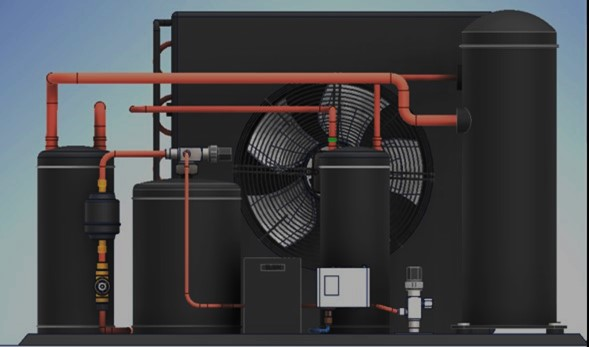
\includegraphics[width=\textwidth]{figures/design-enfria2.jpg}};
		\fill [white,path fading=south] (-5,-4) rectangle (5,4);
		\node[black,font=\Huge\bfseries] at (0,3) {Capítulo III. Meta diseño};
		\node[black,font=\Large\bfseries] at (0,1) {Diseño preliminar del proyecto};
	\end{tikzpicture}
\end{titlepage}




\newpage 
\section*{Introducción}
\addcontentsline{toc}{section}{Introducción}\rsp
\setcounter{chapter}{3}
\setcounter{section}{0}
\setcounter{figure}{0}
\setcounter{page}{35}
\setcounter{table}{0}

El diseño óptimo de frigoríficos usados en la industria para enfriar y congelar productos cada vez más requieren urgentemente de, (i) información técnica de los diversos sistemas existentes, de sus componentes así como de sus aspectos técnicos y operativos del mismo equipo; (ii) memorias de cálculos de análisis energético y exergético para optimizar el diseño del sistema; (iii) uso de las metodologías de refrigeración correctas, (iv) análisis del rendimiento de los componentes; (v) análisis de datos de refrigeración para el diseño de estos mismos sistemas existentes \cite{Dincer2010-re}. 

Derivado de lo anterior, en este capítulo se abordan los fundamentos del diseño óptimo de una cámara de refrigeración para el almacenamiento de insulina, considerada como una parte crítica en la cadena de suministro de medicamentos sensibles a la temperatura. Se hace hincapié en la necesidad de un enfoque multidisciplinario y colaborativo para abordar los desafíos relacionados con el almacenamiento de insulina y se destacan las oportunidades futuras para la mejora continua y la innovación en este campo crucial de la atención médica.

Comprender los principios fundamentales de la preservación de la eficiencia y el diseño de cámaras frigoríficas en ingeniería es esencial para garantizar la integridad y la eficacia de la insulina, un medicamento vital para millones de personas con diabetes en nuestro país.

En el desarrollo de este capítulo, se presenta una estructura clara y detallada para abordar la complejidad de esta tarea. En primer lugar, se analiza exhaustivamente la problemática específica que se busca resolver con este proyecto de ingeniería, centrada en la falta de equipo frigorífico para insulina en la Unidad Médica Familiar 40, ubicada en Azcapotzalco, Ciudad de México. Esta carencia no solo representa un desafío logístico, sino que también compromete la calidad y la eficacia del tratamiento para los pacientes que dependen de este medicamento para controlar su enfermedad (la diabetes).

A continuación, se ahonda en las herramientas del diseño, explorando aspectos técnicos clave para comprender mejor el problema y la solución propuesta. Este análisis incluye la evaluación de requisitos de temperatura, capacidad de almacenamiento, eficiencia energética y otros aspectos relevantes para el diseño y funcionamiento óptimo de la cámara de refrigeración.

Luego, se detallan postulados o marcos de referencia relevantes para la solución de la problemática. Desde el manejo adecuado y seguro de la insulina hasta conceptos teóricos avanzados en el campo de la refrigeración, esta sección proporciona un contexto teórico sólido para informar el diseño y la implementación de la solución.

El cuarto apartado se centra en el ecodiseño, destacando la importancia de considerar criterios de eficiencia y sostenibilidad ambiental en todas las etapas del proceso de diseño y fabricación. Al abordar estos aspectos desde el inicio del proyecto, se busca minimizar el impacto ambiental del sistema de refrigeración y promover prácticas responsables en el uso de recursos naturales.

Seguidamente, se presentan las restricciones técnicas, tanto internas como externas, que deben tenerse en cuenta en soluciones de ingeniería de este tipo. Desde la confiabilidad y seguridad del sistema hasta las políticas y regulaciones que rigen su implementación, estas restricciones juegan un papel crucial en la viabilidad y el éxito del proyecto.

En el sexto apartado, se examinan las regulaciones normativas y legales relacionadas con el diseño de ingeniería y el manejo de la insulina como medicamento destinado al uso de pacientes con diabetes. Cumplir con estas regulaciones es fundamental para garantizar la calidad y seguridad del sistema de refrigeración, así como para mantener la integridad de los medicamentos almacenados.

Posteriormente, se proporciona un bosquejo general del proyecto y su listado de componentes, detallando los elementos clave que formarán parte de la solución final. Esto incluye desde los componentes mecánicos y eléctricos hasta los sistemas de monitoreo y control que garantizarán el funcionamiento eficiente y confiable de la cámara de refrigeración.

Cabe mencionar que gran parte del trabajo desarrollado en este capítulo se logró de manera eficiente por la ayuda otorgada por el Coordinador de Farmacia Familiar en la Unidad Médica Familiar 40, el señor David Ledesma.

Finalmente, se presentan las conclusiones, resumiendo los hallazgos clave y destacando la importancia del desarrollo de este capítulo en el contexto más amplio del proyecto. \rsp
\newpage


\section{Identificación y estructuración de la necesidad detectada}\rsp
\subsection{Necesidad básica}
Los requerimientos son inherentes a cualquier entidad biológica y se refieren a una percepción generada por la noción de carencia, ya sea en términos materiales, físicos o emocionales. Constituyen uno de los pilares esenciales de la existencia, no solo del ser humano sino también de otras formas de vida. Es la exigencia la que impulsa a los organismos a emprender acciones en búsqueda de metas que les permitan cubrir aquello que consideran necesario.
En este sentido, una carencia tecnológica se describe como la discrepancia entre la tecnología existente y la necesaria para potenciar el rendimiento y la competitividad del sector industrial \cite{marrelli-2011,imp-2018}.

 En el contexto del sistema de refrigeración para la conservación de insulina, la necesidad tecnológica se centra en la falta de equipos frigoríficos adecuados para garantizar la estabilidad y eficacia de la insulina almacenada en  la Unidad Médica Familiar 40 (U.M.F 40) en Azcapotzalco, Ciudad de México.
\subsection{Metodología de identificación de la necesidad}
La identificación de las necesidades tecnológicas se llevó a cabo mediante una entrevista personal con Ledesma D. Coordinador de Farmacia Familiar en la U.M.F 40 el día 03 de mayo de 2024 en las instalacione de dicha unidad. En esta visita se recabó información de manera exhaustiva de la situación actual en la unidad, así como a través de un par de consultas con profesionales de la salud dentro de esta misma unidad. Se realizaron visitas al lugar para evaluar las condiciones de almacenamiento de insulina y se recopiló información sobre los problemas y desafíos existentes.


\subsection{Necesidades tecnológicas específicas}
De acuerdo a la entrevista ya mencionada y las visitas realizadas en más de una ocasión, se enlistan algunas de las carencias tecnológicas que se han detectado al interior de la farmacia de medicina familiar y en la red de frío de la U.M.F 40.
\begin{enumerate}
\item Infraestructura: Falta de equipos frigoríficos adecuados y mantenidos para mantener la temperatura requerida para la conservación de insulina. "Se cuenta con una sola unidad de refrigeración para insulina con más de 20 años operando".  
\item Conocimiento: Escasez de información o capacitación sobre el diseño y operación de sistemas de refrigeración para la conservación de insulina. "Solo dos personas aquí entendemos qué pasa internamente con la cámara cuando deja de funcionar". 
\item Metodologías de trabajo: Falta de procedimientos estandarizados para la gestión y distribución de insulina en unidades médicas- "La logistica realmente está en otros hospitales, entonces muchas veces el personal actúa según sus criterios o conocimientos". \cite{david-umf}
\item Herramientas: Carencia de tecnología de refrigeración específicamente diseñada y adaptada para las necesidades de conservación de insulina en entornos médicos. "Como ya se mencionó, el equipo con el que se cuenta es demasiado obsoleto". \cite{david-umf}

\end{enumerate}\rsp
\section{Interrogantes del diseño artefactual}\rsp
Tener un compendio de preguntas en base al diseño que se desee realizar, sirven como herramientas fundamentales para comprender, evaluar y mejorar el proceso de creación de equipos de ingeniería con propósitos específicos. Estas preguntas también servirán de guía en el camino del diseño.\\[-1cm]

\begin{enumerate}
	\item ¿\textit{Cuál es el producto y/o artículo que se va a manejar}?\\ De acuerdo a la información recabada en la visita a la unidad 40 del IMSS se sabe que a los pacientes diabéticos se les proporciona dos tipos de insulina para su tratamiento, \textbf{Humalog Insulina Lispro} Figura \ref{fig:lispro-insul} e \textbf{Insulina Lantus}  Figura \ref{fig:lantus-insul}, este par de medicamentos se suministran directamente por parte del gobierno por lo que la logistica del proceso en la cadena de suministro está debidamente regulada. 
	
	Nota: 100 u/ml es el equivalente para 100 unidades/mililitros por solución inyectable en un vial para ambos productos. Como se aprecia en las cuadros de información. (Vea Cuadros  \ref{tabla:humalog} y \ref{tabla:lantus})  las magnitudes de medida y envasado son muy similares en ambos medicamentos de distinta marca, pero se consideran para cuestiones cálculos de capacidad en el siguiente capítulo.\rsp
		
\begin{table}[H]
	\centering
		\caption{Características de Humalog Insulina lispro. }\cite{lispro-2006}
	\begin{tabular}{ll}
	\toprule
		\textbf{Característica}     & \textbf{Humalog Insulina lispro (100  u/ml )} \\ \midrule
		Peso                        & 100g             \\ % \hline
		Tipo de envasado            & Caja + frasco de vidrio ($12cm\times 3{.}5cm$)     \\ %\hline
		Rendimiento                 & Alta                             \\% \hline
		Precisión                   & (>95\%)                                 \\ %\hline
		Refrigeración       &  Entre 2$^\circ$C y 8$^\circ$C                           \\% \hline
		Tipo de producto & Líquido en frasco de vidrio ambar DIN18\\\bottomrule
	\end{tabular}
	\label{tabla:humalog}
\end{table}\rsp
\begin{table}[H]
	\centering
	\caption{Características de Lantus Insulina Glargina}\cite{lantus-2015}
	\begin{tabular}{ll}
	\toprule
	\textbf{Característica}     & \textbf{Lantus\textsuperscript{\textregistered} Insulina} \\ \midrule
	Peso                        & 100g             \\ % \hline
	Tipo de envasado            & Caja + frasco de vidrio  ($12cm\times 3{.}5cm$)     \\ %\hline
	Rendimiento                 & Alta                             \\% \hline
	Precisión                   & (>95\%)                                 \\ %\hline
	Refrigeración       &  Entre 2$^\circ$C y 8$^\circ$C                            \\% \hline
	Tipo de producto & Líquido en frasco ampula\\ \bottomrule
\end{tabular}
	\label{tabla:lantus}
\end{table}
\newpage
\begin{multicols}{2}
 
\begin{figure}[H]
	\centering
	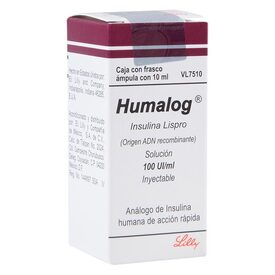
\includegraphics[width=0.6\linewidth]{figures/lispro-insul}
	\caption{Envase de insulina Humalog 10ml}
	\label{fig:lispro-insul} Fuente: \cite{sanpablo}
\end{figure}
\begin{figure}[H]
	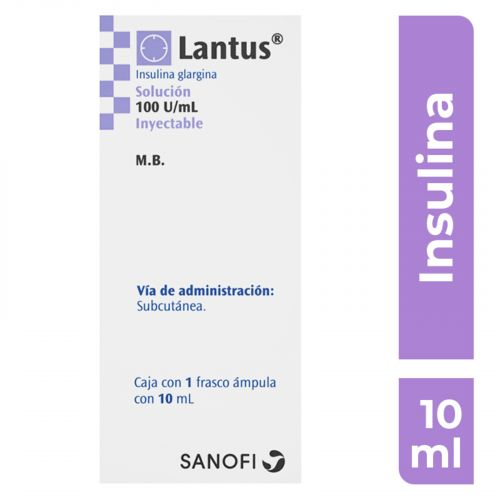
\includegraphics[width=0.6\linewidth]{figures/lantus-insul}
	\caption{Envase de insulina Lantus 10ml}
	\label{fig:lantus-insul}   Fuente: \cite{ahorro}
\end{figure}

\end{multicols}
 



	\item \textit{¿Qué tipo de producción se va a realizar?}\\
	El principal motivo de la cámara frigorífica será la \textbf{conservación de la insulina}, específicamente los dos tipos de insulina ya descritos. También el proceso de conservación implica actividades como las que se mencionan en la pregunta 5.	Estas actividades de producción se centran en asegurar que la insulina se mantenga en condiciones óptimas para su uso seguro y efectivo en el tratamiento de la diabetes.
	
	\item \textit{¿Qué tipo de línea de producción?}\\
En el caso de la conservación de insulina, se usará \textbf{una línea de producción específica} y dedicada exclusivamente a este medicamento. Es fundamental evitar la mezcla de insulina con otros productos farmacéuticos debido a razones de seguridad y eficacia. La insulina es un medicamento vital para el tratamiento de la diabetes, y cualquier contaminación cruzada o confusión en su distribución puede tener consecuencias graves para la salud de los pacientes. Además, el manejo de múltiples productos en la misma línea de producción aumenta el riesgo de errores humanos y puede comprometer la calidad y pureza del medicamento. Por lo tanto, se recomienda encarecidamente que la línea de producción de insulina se mantenga separada y dedicada exclusivamente a este medicamento, garantizando así la seguridad y eficacia de su producción y distribución. \cite{david-umf}
	\item \textit{¿Qué condiciones ambientales se requieren?}\\
	Dado que el equipo frigorífico está destinado para ubicarse en la U.M.F 40, se tomarán variables metereológicas de la Ciudad de México espacialmente ubicándose en las coordenadas de la alacaldía Azcapotzalco, puesto que en \cite{cressie-1993} se menciona que las variables medidas espacialmente tienen dependencia y correlación es válido tomar datos medidos a nivel general de la CDMX. (Vea Cuadro \ref{tabla:clima}) 
	 
		
		 
			\begin{table}[H]
				\centering
				\caption{Resumen de información sobre el clima y características del valle de México.}\cite{weather-cdmx}
				\begin{tabular}{p{5cm}p{7cm}}
					\toprule
					\textbf{Información} & \textbf{Detalle} \\
					\midrule
				\begin{center}
					 \vspace*{0.5cm}Clima
				\end{center}	 & 
					\begin{itemize}
						\item Templado subhúmedo: 87\%
						\item Seco y semiseco: 7\%
						\item Templado húmedo: 6\%
					\end{itemize} \\
					%\midrule
					Temperatura media anual & 16°C \\
					%\midrule
					\begin{center}
						\vspace*{0.5cm} Temperaturas extremas
					\end{center}	
					 & 
					\begin{itemize}
						\item Más alta (>25°C): marzo a mayo
						\item Más baja (alrededor de 5°C): enero
					\end{itemize} \\
					%\midrule
					\begin{center}
						\vspace*{0.5cm}Precipitación total anual
					\end{center}	
					 & 
					\begin{itemize}
						\item Región seca: 600 mm
						\item Parte templada húmeda: 1 200 mm
					\end{itemize} \\
				%	\midrule
					\begin{center}
						\vspace*{0.5cm}Ecosistemas
					\end{center}	 & Avance de la mancha urbana ha puesto en peligro todos los ecosistemas, especialmente los lagos. \\
					%\midrule
					\begin{center}
						\vspace*{1.2cm}Uso de suelo
					\end{center}	 & 
					\begin{itemize}
						\item Zona urbana: mayor parte del territorio
						\item Zonas agrícolas: principalmente al sur y sureste, con cultivos de maíz, frijol, avena, nopal, hortalizas y floricultura.
					\end{itemize} \\
					\bottomrule
				\end{tabular}
				\label{tabla:clima}
			\end{table}
		 
		
	\item \textit{¿Cual es el proceso de trabajo que tiene que realizar el sistema artefactual?}
	\begin{itemize}
		\item Recepción: Ingreso de la insulina como penúltimo punto de la cadena de suministro descrita en la \hyperlink{figura-2-15}{figura 2.15} para poder ser entregada al paciente cuando lo solite. 
		\item Pre-enfriamiento: Reducimos la temperatura del medicamento y mantenemos en un valor fijo de temperatura, la cual se decide en cuestión del consumo energético de la zona.
		\item Almacenar: Mantener la insulina a la temperatura adecuada (2$^\circ$C a 8$^\circ$C) para garantizar su estabilidad y eficacia .
		\item Conservar: Proteger la insulina de condiciones ambientales adversas que puedan afectar su calidad, en nuestro caso los sismos (temblores).
		\item Supervisar: Monitorizar constantemente la temperatura y otras condiciones dentro de la cámara para asegurar que se mantengan dentro de los rangos aceptables, se adjuntará un sensor de temperatura para que cuando la temperatura en el sistema comience a subir este baje la temperatura a 2$^\circ$C nuevamente.
		\item Registrar: Mantener registros precisos de los niveles de inventario, fechas de vencimiento y otros datos relevantes para el seguimiento y la trazabilidad del producto. Actividades destinadas al personal para control interno y para temas de mantenimiento del equipo.
		\item Organizar: Distribuir y organizar la insulina de manera eficiente dentro de la cámara para facilitar su acceso y manejo. Se dispondrán de divisiones horizontales comunes para poder diferenciar ambas marcas de insulina. 
	\end{itemize}		
	\item \textit{¿Cuántas etapas de trabajo tiene que realizar el sistema artefactual?}\\
	Según \citeauthor{cengel-2009}\citeyear{cengel-2009},  el ciclo real de refrigeración por compresión consta de los siguientes procesos vea Figura la \ref{ciclo-ref}: evaporación, compresión, condensación y expansión, por lo cual siguiendo este ciclo se destinarán las etapas de trabajo que va a realizar nuestro sistema. Entonces el diseño realizará \textbf{6 etapas} para llevar a cabo la refrigeación y conservación de la insulina.
	
	% revisar aquí en futuro para mejorar
	\begin{enumerate}
		\item[i)] Inicio del Sistema: Cuando se enciende el sistema de refrigeración, el compresor es el primer componente en activarse. El compresor es el motor del sistema y su función es comprimir el refrigerante gaseoso.
		\item[ii)] Compresión del Refrigerante: El compresor aumenta la presión y la temperatura del refrigerante gaseoso. Este proceso demanda una cantidad considerable de energía, especialmente para superar la resistencia de la compresión.
		\item[iii)] Transferencia de Calor en el Condensador: El refrigerante comprimido se dirige hacia el condensador, donde cede calor al entorno circundante. El condensador, un intercambiador de calor, convierte el refrigerante gaseoso en líquido al disipar el calor hacia el exterior.
		\item[iv)] Expansión del Refrigerante en la Válvula de Expansión: Después de enfriarse en el condensador, el refrigerante pasa a través de la válvula de expansión. Esta válvula reduce la presión del refrigerante y lo dirige hacia un conducto más estrecho, lo que resulta en una rápida disminución de la temperatura.
		\item[v)] Absorción de Calor en el Evaporador: El refrigerante líquido y frío ingresa al evaporador, donde absorbe el calor del entorno interior de la cámara de refrigeración. Durante este proceso, el refrigerante se evapora y extrae calor del ambiente, manteniendo así una temperatura baja en el interior de la cámara.
		\item[vi)]Retorno del Refrigerante al Compresor: Una vez que el refrigerante ha absorbido el calor, regresa al compresor en forma de vapor para reiniciar el ciclo de refrigeración.
	\end{enumerate}
	Durante todo este proceso, diversos componentes del sistema, como los tubos y conexiones, el aceite lubricante, los controladores y sensores, y el aislamiento, colaboran para garantizar un funcionamiento eficiente y confiable. \cite{neoattack-2023,cengel-2009}
	
	\begin{figure}[H]
		\centering
		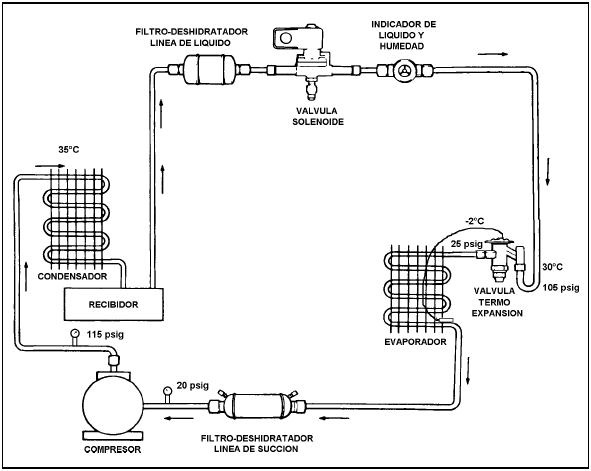
\includegraphics[width=0.5\linewidth]{figures/ciclo-ref}
		\caption{Diagrama de un sistema de refrigeración típico con R-134a}
		\label{fig:ciclo-ref} Fuente: \cite{agustin}
	\end{figure}
	
	
	\item \textit{¿El diseño del sistema artefactual puede ser modular y flexible?}
	\textbf{Sí} De acuerdo con los sitios web de las empresas \citeauthor{hogartecnocasa-2016} y \citeauthor{neoattack-2023} un sistema modular es aquél que puede ser manipulado mendiante un ordenador o software especializado y que en sí mismo puede ser dividido en sistemas más pequeños, en los cimientos de este proyecto es un aspecto que no se considerará como parte del estudio por las premuras del tiempo, sin embargo es algo que sin duda puede considerarse. No obstante el proyecto en cuestión sí que es flexible por sus dimensiones que serán designadas bajo un análisis profundo en el siguiente capítulo. 
	
	
\item 	\textit{¿Se puede aplicar la inteligencia artificial y la robotización en el sistema?}\\
\textbf{Sí}, es factible aplicar tanto la inteligencia artificial (IA) como la robotización en un sistema de refrigeración destinado a la preservación de la insulina. Estas tecnologías pueden aportar una serie de ventajas significativas en términos de eficiencia, automatización y optimización del rendimiento del sistema. En \citeauthorNP[et. al.]{madriz-ramirez-2022} \citeyear{madriz-ramirez-2022}, se ha trabajado en un diseño especializado en refrigeración que resulta novedosa y práctica, este es un ejemplo práctico de como técnicas modernas pueden coadyuvar a mejorar la eficiencia y optimización de proyectos en ingeniería que a lo largo de los años han ido adaptándose también y como era de esperarse la ingeniería mecánica aplicada a los sistemas de refrigeración no serían la excepción.

\item 	\textit{¿Cómo podemos aprovechar las nuevas fuentes de datos?}\\
El gran campo que se ha creado entorno a los datos era conocida como "big data" por los investigadores sin lugar a dudas puede ser de gran utilidad para el diseño óptimo de sistemas de refrigeración ya que de bases de datos históricas podemos determinar el tiempo de fallo de componentes o tiempos de vida útil, así como de ellas se pueden sacar ventajas para la predicción de la falla de componentes, la monitorización en tiempo real también puede ser una herramienta novedosa aplicada al campo de estudio que conciernea este proyecto. Finalmente en el siguiente artículo  hecho por investigadores de China muestran estudios de lo potenciales que pueden ser estas nuevas bases de datos y modelos en monitorización de temperaturas en distintas temporadas del año, vea \cite{liu-2021} para más detalles.


\item	Conexión a un HOST (computadoras, tabletas móviles, portátiles)\\
De igual manera, la conexión a estos dispositivos que cada día son más frecuentes en el uso cotidiano sin dudarlo ayudarían mucho a los sistemas de vigilancia remotas en tiempo real del sistema de refrigeración, por ejemplo en tiempos de epidemia en donde el contacto con material de salud suele ser muy delicado para evitar contagios se pueden aplicar a la regulación de la temperatura y de humedad desde algún dispositivo móvil.



\item 	¿Se puede aplicar el desmantelamiento y reciclado del sistema al ciclo de uso?
Esta es una de las problemáticas principales que se siguen trabajando en los diseños de ingeniería en el campo farmaceútico, debido a que por normas oficiales los instrumentos y equipos de trabajo destinados a la salud pública tienen estrictamente prohibido la reutilización en actividades que no sean internas de la instancia de gobierno (clínica, UMF, hospitales, etc), sin embargo es claro que para fines del mismo equipo con autorización de expertos en área de salud y diseño farmaceútico estos componentes o equipos pueden ser reutilizados en un equipo nuevo o averiado.
	
\end{enumerate}


\section{Marco teórico }


La insulina, al igual que otros fármacos basados en hormonas peptídicas, está sujeta a la influencia de las condiciones ambientales, lo cual impacta su estabilidad y eficacia terapéutica. A pesar de la omnipresencia de la insulina en múltiples etapas de la cadena de suministro y su uso diario por personas con diabetes, existe una notable falta de investigación sobre cómo varía su potencia durante la cadena de frío y hasta el momento de su administración.

Para garantizar la calidad y eficacia de la insulina, es fundamental comprender cómo el calor y el frío afectan su estabilidad. Las recomendaciones de almacenamiento reflejan la importancia de mantener condiciones específicas de temperatura para preservar la integridad del medicamento. Sin embargo, la falta de datos públicos sobre la estabilidad de la insulina y su potencia en diferentes condiciones de almacenamiento dificulta la evaluación de los riesgos asociados con su uso.  \textcolor{white}{ \citeyearNP{heinemann-2020}} \cite{heinemann-2020}

 Además, mejorar la eficiencia energética en sistemas de refrigeración es crucial, especialmente considerando que los sistemas HVAC\&R son notoriamente grandes consumidores de energía. La adopción de tecnologías más ecológicas, como compresores de corriente continua y el uso de energías renovables, ofrece oportunidades significativas para reducir costos y minimizar el impacto ambiental de estos sistemas. Investigaciones en este campo están en curso, buscando desarrollar sistemas de refrigeración más eficientes y sostenibles.
 
 Por último, en el diseño de cámaras de refrigeración, es esencial tener en cuenta tanto los cálculos teóricos como la teoría detrás de los principios de refrigeración. Esto garantiza que las cámaras cumplan con los estándares de temperatura necesarios para preservar la integridad de los productos farmacéuticos, como la insulina, y mantener la eficiencia energética de los sistemas de refrigeración. Un diseño bien fundamentado asegura un almacenamiento adecuado y seguro de medicamentos sensibles a la temperatura, contribuyendo así a la salud y bienestar de los pacientes. \cite{parise-2005}


	\subsection{Carga del producto }	

En la termodinámica clásica, nos interesan principalmente los cambios y las transferencias de energía y masa entre ciertos cuerpos (por ejemplo, un tanque de agua o una cantidad de gas, etc.). Para clarificar las discusiones, llamamos al cuerpo particular de interés (o región del espacio) el sistema. El sistema a menudo (pero no necesariamente) está contenido dentro de algún límite físico. Cuando el límite del sistema permite que la materia (masa) entre o salga del sistema, se dice que es un sistema abierto. Cuando el límite del sistema no permite que la masa entre o salga del sistema, pero permite que el trabajo y/o el calor se transfieran a través del límite, se dice que es un sistema cerrado. En el caso inusual de que el límite del sistema no permita que ni la masa ni la energía (en forma de calor o trabajo) crucen el límite, se dice que es un sistema aislado.

La distinción entre sistemas abiertos y cerrados es importante, ya que los análisis termodinámicos de sistemas cerrados tienden a ser más simples, debido al hecho de que no tenemos que considerar los cambios en la energía de un sistema producidos simplemente por la transferencia de masa con su energía intrínseca dentro o fuera del sistema. Este es el caso del refrigerante en un refrigerador o bomba de calor (siempre que no haya fugas), y por lo tanto solo necesitamos considerar los efectos de transferencia de trabajo y calor. \cite{james-2013}

De acuerdo con \citeauthor{bohn}, \citeyear{bohn} algunas consideraciones importantes para el diseño frigorífico en base un producto perecedero la carga de producto recae en lo siguiente. 
\begin{enumerate}
	\item Cuando un artículo se introduce en una cámara de refrigeración o congelación, su temperatura disminuye hasta alcanzar la temperatura deseada, (vea el \hyperref[anexo:bohn-perecederos]{anexo 4})  , para conocer algunas características comunes a considerar en el diseño. Este proceso involucra tres componentes de carga térmica:
	\begin{enumerate}
		\item El calor específico se refiere a la cantidad de calor que se debe extraer de una libra de producto para reducir su temperatura en 1°F. Este valor varía dependiendo de si el producto está por encima o por debajo del punto de congelación.
		\item El calor latente, conocido como calor de fusión, es la cantidad de calor que se debe eliminar para congelar una libra de producto. La mayoría de los productos tienen un punto de congelación típico, y se puede estimar en 28°F si no se conoce exactamente.
		\item La respiración es el calor generado por frutas y verduras frescas mientras están almacenadas, debido a su actividad metabólica. Este calor varía según el tipo y la temperatura del producto y se mide en unidades BTU por libra por día.
	\end{enumerate}
	\item Cuando se calcula la carga del producto con un tiempo de abatimiento diferente a 24 horas, se debe aplicar un factor de corrección, que es la relación entre 24 horas y el tiempo de abatimiento, a la carga del producto.
	\item Es importante tener en cuenta que, aunque se pueda calcular el abatimiento de temperatura del producto, no se puede garantizar la temperatura final debido a diversos factores externos e incontrolables, como el tipo de empaque, la posición de la carga y el método de almacenamiento.
\end{enumerate}
\subsection{Cargas térmicas de climatización}
Es importante para el control clínico de la insulina mantener adecuadas la temperatura y la humedad en condiciones ideales para la preservación segura de este medicamento.

El análisis de las cargas térmicas es un proceso llevado a cabo por expertos para evaluar las demandas de climatización de un entorno, sin importar su propósito, ya sea residencial, comercial o industrial.
La carga térmica se refiere a la cantidad de energía requerida para mantener o alcanzar ciertas condiciones de temperatura y humedad en un espacio específico, adaptándose a su uso particular, ya sea en un hogar para determinar las necesidades de calefacción, o en un almacén de alimentos congelados para garantizar sistemas de refrigeración confiables. \cite{sampp-2023}
\subsubsection{Cargas sensibles}
Las cargas sensibles incluyen la transmisión de calor a través de los cerramientos
opacos y traslúcidos, la radiación solar, la ventilación o infiltración de aire, la
ocupación del local, la iluminación y la maquinaria presente en el espacio.

\begin{itemize}
	\item \textbf{Cargas por transmisión a través de cerramientos opacos}
\begin{equation} \label{eq:carga_transmision_opacos}
	Q = U \cdot A \cdot \Delta T
\end{equation}
Siendo:
\begin{align*}
	Q & : \text{carga térmica por transmisión (W)} \\
	U & : \text{transmitancia térmica del muro (W/m}^2 \, ^\circ\text{C)} \\
	A & : \text{superficie del muro expuesta a la diferencia de temperaturas (m}^2\text{)} \\
\Delta T & : \text{diferencia de temperaturas, corregida según la orientación del muro y su peso}
\end{align*}

\item \textbf{Cargas por transmisión a través de cerramientos traslúcidos}
\begin{equation} \label{eq:carga_transmision_traslucidos}
	Q = U \cdot A \cdot \Delta T
\end{equation}
Donde:
\begin{align*}
	\Delta T & : \text{diferencia de temperaturas entre las caras interior y exterior del cerramiento (}^\circ\text{C)}
\end{align*}

\item \textbf{Cargas térmicas por radiación solar}
\begin{equation} \label{eq:carga_radiacion_solar}
	Q = S \cdot R \cdot f
\end{equation}
Siendo:
\begin{align*}
	S & : \text{superficie traslúcida expuesta a la radiación (m}^2\text{)} \\
	R & : \text{radiación solar que atraviesa un vidrio sencillo (W/m}^2\text{)} \\
	f & : \text{factores de corrección de la radiación en función del tipo de vidrio}
\end{align*}
En la tabla \ref{table:carrier} se dan los valores de las máximas aportaciones solares a través de vidrio sencillo.\\
En cuanto a los coeficientes de corrección $f$, los que se aplican habitualmente son el de marco metálico ($f = 1{.}17$) y el factor solar del vidrio, que los fabricantes indican en sus fichas técnicas como $g$. En caso de que queramos aplicar dos coeficientes de corrección, deberemos multiplicarlos.
\item \textbf{Carga sensible por ventilación o infiltración de aire exterior}

\begin{equation} \label{eq:carga_ventilacion_infiltracion}
	Q = V \cdot 0{.}34 \cdot \Delta t
\end{equation}
Donde:
\begin{align*}
	V & : \text{caudal de aire infiltrado o de ventilación (m}^3/\text{h)} \\
	\Delta t & : \text{diferencia de temperatura entre el ambiente exterior y el interior (}^\circ\text{C)}
\end{align*}

\begin{table}[H]
	\centering
	\caption{valores de las máximas aportaciones solares a través de vidrio sencillo } Fuente: \cite{carrier-1980}
	\begin{tabular}{@{}lcccccccccc@{}}
		\toprule
		& \multicolumn{1}{l}{} & \multicolumn{9}{c}{Orientación}                                             \\ \midrule
		& \multicolumn{1}{l}{} & \multicolumn{9}{c}{Máximas aportacionas solares R (W/m\textasciicircum{}2)} \\ \cmidrule(l){3-11} 
		\multicolumn{1}{c}{Latitud Norte} & Mes                  & N     & NE     & E      & SE     & S     & SO    & O     & NO    & Horiz.   \\ \midrule
		\multirow{3}{*}{}                 & Junio                & 63    & 437    & 506    & 283    & 66    & 283   & 506   & 437   & 786      \\
		& Julio y Mayo         & 50    & 412    & 515    & 314    & 94    & 314   & 515   & 412   & 774      \\
		& Agosto y Abril       & 34    & 339    & 519    & 405    & 197   & 405   & 519   & 339   & 739      \\
		\multicolumn{1}{c}{30°}           & Sept.y Marzo         & 28    & 283    & 496    & 478    & 329   & 478   & 496   & 283   & 666      \\
		& Oct. y Febrero       & 24    & 122    & 425    & 513    & 456   & 513   & 425   & 122   & 563      \\
		& Nov. y Enero         & 22    & 50     & 364    & 509    & 500   & 509   & 364   & 50    & 456      \\
		& Diciembre            & 19    & 37     & 329    & 509    & 513   & 509   & 329   & 37    & 412      \\ \midrule
		& Junio                & 53    & 418    & 509    & 349    & 169   & 349   & 509   & 418   & 745      \\
		& Julio y Mayo         & 46    & 399    & 515    & 393    & 217   & 393   & 515   & 399   & 732      \\
		& Agosto y Abril       & 34    & 320    & 509    & 458    & 320   & 459   & 509   & 320   & 673      \\
		\multicolumn{1}{c}{40°}           & Sept.y Marzo         & 28    & 182    & 469    & 509    & 440   & 509   & 469   & 182   & 575      \\
		& Oct. y Febrero       & 22    & 109    & 383    & 513    & 509   & 513   & 383   & 109   & 405      \\
		& Nov. y   Enero       & 15    & 37     & 314    & 491    & 522   & 491   & 314   & 37    & 324      \\
		& Diciembre            & 15    & 31     & 270    & 465    & 519   & 465   & 270   & 31    & 267      \\ \bottomrule
	\end{tabular}
\end{table}
	El siguiente escenario fue realizado bajo una temperatura ambiente constante de 43ºC, sin la presencia de productos en su interior. Como se evidencia en la figura \ref{fig:cargas-ter} la pendiente de la carga térmica en el conservador es mayor en el congelador. Este comportamiento se debe principalmente a las dimensiones del conservador las cuales dan lugar a un mayor intercambio de aire con el entorno circundante a la nevera.  \cite{rio}


\begin{figure}[H]
	\centering
	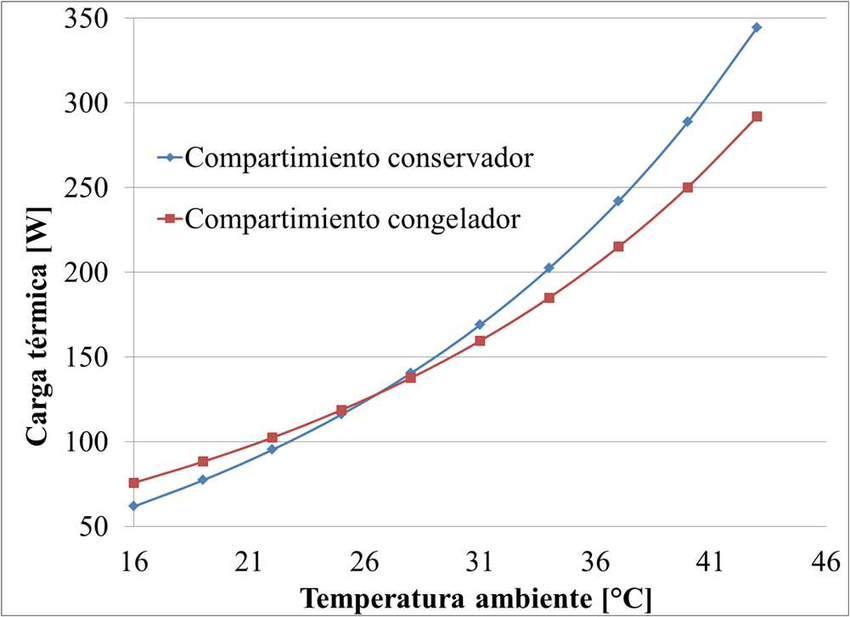
\includegraphics[width=0.46\linewidth]{figures/cargas-ter}
	\caption{Carga térmica vs humedad relativa}
	\label{fig:cargas-ter} Fuente: Este experimento fue realizado por \citeNP{rio}
\end{figure}




\label{table:carrier}
\begin{itemize}
	\item \textbf{Cargas generadas por la iluminación del local}
	
	Se considerará que la potencia integrada de la lámpara se transformará en calor sensible; en el caso de las lámparas de descarga (fluorescentes) se incrementará el valor obtenido en un 25\% para tener en cuenta el cebador y el balasto.	
	\item \textbf{Lámparas incandescentes o LED} 
	\begin{equation} \label{eq:carga_iluminacion_incandescente}
		Q =  {Pot}
	\end{equation}	
	\item \textbf{Lámparas de descarga} 
	\begin{equation} \label{eq:carga_iluminacion_descarga}
		Q = 1{.}25 \cdot {Pot}
	\end{equation}	
	 {Donde:}
	\begin{align*}
		Q & : \text{carga térmica por iluminación (W)} \\
		 {Pot} & : \text{potencia de las lámparas (W)}
	\end{align*}
	\item \textbf{Cargas generadas por las máquinas presentes en el local}
	
	Se considerará que las pérdidas de la maquinaria se transforman íntegramente en calor sensible.	
\item \textbf{Carga generada por maquinaria} 
	\begin{equation} \label{eq:carga_maquinaria}
		Q = \eta \cdot {Pot}
	\end{equation}
	
	 {Donde:}
	\begin{align*}
		Q & : \text{carga térmica por maquinaria (W)} \\
		\eta & : \text{rendimiento de la máquina} \\
		\text{Pot} & : \text{potencia de la maquinaria (W)}
	\end{align*}
\end{itemize}
\subsubsection{Cargas latentes}
\begin{itemize}
	
	\item \textbf{Carga latente por ventilación o infiltración de aire exterior}
	\textbf{Carga latente de ventilación o infiltración.}
	\begin{equation} \label{eq:carga_latente_ventilacion}
		Q = V \cdot 0.63 \cdot \Delta w
	\end{equation}
	
	 {Donde:}
	\begin{align*}
		Q & : \text{carga térmica latente por ventilación o infiltración de aire (W)} \\
		V & : \text{caudal de aire infiltrado o de ventilación (m}^3/\text{h)} \\
		\Delta w & : \text{diferencia de humedad absoluta entre el ambiente exterior y el interior (ºC)}
	\end{align*}
	
\item \textbf{Carga latente por ocupación del local}
	
	Esta carga se determina multiplicando una valoración del calor latente emitido por la persona tipo por el número de ocupantes previstos para el local. La cantidad de calor emitido por persona se obtiene de la tabla que aparece en el apartado donde se describe la Carga sensible por ocupación del local.
	
\end{itemize}
Las formulas descritas se tomaron de \cite{bruno-2024,carrier-1980,sampp-2023}\rsp
\end{itemize}
\section{Ecodiseño}\rsp
El reglamento de ecodiseño se aplica a una amplia gama de equipos, incluyendo unidades condensadoras y centrales de compresores para refrigeración a media y baja temperatura. Nuestros productos cumplen con los requisitos establecidos para coeficiente de rendimiento (COP) y rendimiento estacional normalizado (SEPR), este factor es utilizado para comparación de equipos funcionando en modo refrigeración para escenarios de refrigeración para procesos industriales, garantizando así un funcionamiento eficiente y respetuoso con el medio ambiente (vea el cuadro \ref{tabla:condensadores}) \cite{intarcon-2023}.\\
En el caso de las enfriadoras de proceso , los requisitos de ecodiseño se aplican a equipos de cualquier potencia, con enfriamiento por aire o por agua, tanto para media como para baja temperatura (cuadro \ref{tabla:enfriadores-med-baj}). También se han establecido requisitos para las enfriadoras de proceso de alta temperatura, que entrarán en vigor a partir de enero de 2018 y enero de 2021. (cuadro \ref{tabla:enfriadores-alta})\\
Por ejemplo, para unidades condensadoras con una potencia nominal de hasta 5 kW y 2 kW en media y baja temperatura respectivamente, se exige un COP mínimo a partir del 1 de julio de 2016. Este requisito se incrementa para equipos de mayor potencia, donde el SEPR se convierte en el parámetro de referencia.\\
El ecodiseño no solo se limita a cumplir con los estándares de rendimiento energético, sino que también aborda otros aspectos importantes, como la reducción de la carga refrigerante, la sectorización de los sistemas de refrigeración, la minimización del riesgo de fugas y la utilización de refrigerantes de bajo potencial de calentamiento atmosférico. Estas medidas tienen como objetivo reducir el impacto ambiental de los sistemas de refrigeración y promover un futuro sostenible \cite{caloryfrio-2018}.  
\begin{figure}[H]
	\centering
	
\includegraphics[width=0.3\linewidth]{figures/edodis}
	\caption{El Grupo CIAT implementa el Ecodiseño en sus sistemas de climatización y refrigeración.} Fuente: \cite{ciat}
	\label{fig:edodis}
\end{figure}

\begin{table}[H]
	\centering
	\caption{Requisitos de ecodiseño para unidades condensadoras}\cite{intarcon-2023}
	\begin{tabular}{lllcc}
		\toprule
		\textbf{Temperatura} & \textbf{Pot. nominal} & \textbf{Factor} & \textbf{Valor mínimo }  & \textbf{Valor mínimo } \\
		
		 & & & \textbf{desde 01/07/2016} & \textbf{desde: 01/07/2018} \\
		
		\midrule
		Media & $0,2 \, \text{kW} \leq \text{PA} \leq 1 \, \text{kW}$ & COP & 1,20 & 1,40 \\
		& $1 \, \text{kW} < \text{PA} \leq 5 \, \text{kW}$ & COP & 1,40 & 1,60 \\
		& $5 \, \text{kW} < \text{PA} \leq 20 \, \text{kW}$ & SEPR & 2,25 & 2,55 \\
		& $20 \, \text{kW} < \text{PA} \leq 50 \, \text{kW}$ & SEPR & 2,35 & 2,65 \\
		\midrule
		Baja & $0,1 \, \text{kW} \leq \text{PA} \leq 0,4 \, \text{kW}$ & COP & 0,75 & 0,80 \\
		& $0,4 \, \text{kW} < \text{PA} \leq 2 \, \text{kW}$ & COP & 0,85 & 0,95 \\
		& $2 \, \text{kW} < \text{PA} \leq 8 \, \text{kW}$ & SEPR & 1,50 & 1,60 \\
		& $8 \, \text{kW} < \text{PA} \leq 20 \, \text{kW}$ & SEPR & 1,60 & 1,70 \\
		\bottomrule
	\end{tabular}
	\label{tabla:condensadores}
\end{table}


\begin{table}[htbp]
	\centering
	\caption{Requisitos de ecodiseño para enfriadoras de proceso de media y baja temperatura}\rsp 
	\cite{intarcon-2023}
	\begin{tabular}{lllcc}
		\toprule
		\textbf{Condensación} & \textbf{Temperatura} & \textbf{Potencia nominal PA} & \multicolumn{2}{c}{\textbf{Valor mínimo a partir del}} \\
		& & & \textbf{01/07/2016} & \textbf{01/07/2018} \\
		\midrule
		Aire (a 35ºC) & Media (-8ºC) & PA $\leq$ 300 kW & 2,24 & 2,58 \\
		& & PA $>$ 300 kW & 2,80 & 3,22 \\
		&Baja (-25ºC) & PA $\leq$ 200 kW & 1,48 & 1,70 \\
		& & PA $>$ 200 kW & 1,60 & 1,84 \\
		Agua (a 30ºC) & Media (-8ºC) & PA $\leq$ 300 kW & 2,86 & 3,29 \\
		& & PA $>$ 300 kW & 3,80 & 4,37 \\
		&Baja (-25ºC) & PA $\leq$ 200 kW & 1,82 & 2,09 \\
		& & PA $>$ 200 kW & 2,10 & 2,42 \\
		\bottomrule
	\end{tabular}
	\label{tabla:enfriadores-med-baj}
\end{table}

\begin{table}[H]
	\centering
	\caption{Requisitos de ecodiseño para enfriadoras de proceso de alta temperatura}
	\cite{intarcon-2023}
	\begin{tabular}{lllll}
		\toprule
		\textbf{Condensación} & \textbf{Temperatura} & \textbf{Potencia nominal PA} & \multicolumn{2}{c}{\textbf{Valor mínimo a partir del}}\\
		& & & \textbf{01/01/2018}& \textbf{01/01/2021}\\
		\midrule
		Aire (a 35ºC) & Alta (7ºC) & PA $<$ 400 kW & 4.5&5.0 \\
		& & PA $>$ 400 kW & 5&5.5 \\
		Agua (a 30ºC) & Alta (7ºC) & PA $<$ 400 kW & 6,5&7.0 \\
		& & $400 \, \text{kW} \leq \text{PA} < 1500 \, \text{kW}$ & 7.5 &8.0 \\
		& & PA $>$ 1500 kW & 8.0 &8.5 \\
		\bottomrule
	\end{tabular}
	\label{tabla:enfriadores-alta}
\end{table}

\section{Restricciones técnicas internas y externas} \rsp
 \subsection{Factor de Seguridad}
 Después de calcular las cuatro principales fuentes de calor, se agrega un factor de seguridad del 10\% a la carga total de refrigeración. Este factor se incorpora para considerar posibles omisiones o inexactitudes mínimas en los cálculos, proporcionando así una capa adicional de seguridad o reserva que puede provenir del rendimiento del compresor y las fluctuaciones en la carga promedio.
 \subsection{Dimensionamiento y Aislamiento de la Cámara de Refrigeración}
 
 Para realizar el dimensionamiento y aislamiento de la cámara de refrigeración en la Unidad Médica Familiar 40 en Azcapotzalco, CDMX, se seguirán las normas oficiales de México que regulan este tipo de instalaciones, asegurando así el cumplimiento de estándares de calidad y seguridad. A continuación, se detalla el proceso:
 
 \begin{enumerate}
 	\item \textbf{Determinación de requisitos}: Se comenzará identificando los requisitos específicos de la cámara de refrigeración para el almacenamiento de insulina en la Unidad Médica Familiar 40. Esto incluirá el volumen de almacenamiento necesario, la temperatura requerida para mantener la integridad de la insulina, y cualquier otro requisito relevante.
 	
 	\item \textbf{Cálculo de espacio y distribución interna}: Basado en los requisitos identificados, se calculará el espacio necesario y se diseñará la distribución interna de la cámara. Se determinará la disposición de las estanterías y los espacios necesarios para el almacenamiento eficiente de la insulina, teniendo en cuenta factores como el acceso fácil y la circulación del aire.
 	
 	\item \textbf{Selección de materiales y equipos}: Se seleccionarán los materiales adecuados para las paredes, techo y suelo de la cámara, teniendo en cuenta las normas oficiales de México sobre conductividad térmica, resistencia a la humedad y resistencia estructural. Además, se elegirán los equipos de refrigeración, como el evaporador, compresor y condensador, garantizando su compatibilidad con las necesidades de temperatura y espacio de la cámara.
 	
 	\item \textbf{Diseño conceptual y distribución de equipos}: Con base en los cálculos y selecciones anteriores, se elaborará un diseño conceptual detallado de la cámara de refrigeración, se usará software de diseño de ingeniería. Esto incluirá la distribución de los equipos de refrigeración dentro de la cámara, así como la ubicación de la puerta y componentes para facilitar el acceso y la ventilación adecuada.
 	
 	\item \textbf{Consideraciones adicionales}: Se tendrán en cuenta otras consideraciones importantes, como la instalación de sistemas de monitoreo de temperatura y humedad, la instalación de sistemas de respaldo de energía para evitar interrupciones en el suministro de energía, y la implementación de medidas de seguridad para proteger tanto la insulina almacenada como el personal que trabaja en la unidad médica.
 \end{enumerate}

 Y para empezar con el dimensionamiento de la cámara frigorífica, se da a conocer 
 las medidas de cada empaque de la insulina en sus dos versiones, consulte las tablas \ref{tabla:humalog} y \ref{tabla:lantus}, también el peso que puede contener cada
 empaque con el fin de almacenar una cantidad grande de insulina o refrigerar al menos la cantidad promedio de medicamento que llega a la unidad.\\
 Con dicho calculo se procederá a hacer un diseño conceptual, de la cámara donde
 especificará el espacio que se ocupara, la distribución de la estantería, el producto
 a almacenar, así como indicar donde se colocaran las puertas y ventanas, para
 después colocar la distribución del equipo de refrigeración, que son el evaporador,
 compresor, condensador, y todos los equipos adicionales que se requieran para el
 óptimo funcionamiento de nuestra cámara frigorífica.\\
 Después de recabar la información del dimensionamiento obtenemos las cargas térmicas para el equipo en base a la sección 3.3.2 en este capítulo. Además consideramos las cargas que afectan la temperatura del sistema, las cuales son
 
 \subsubsection{Cargas por conducción en paredes y techo}
 
 Los paredes y techos de las cámaras frigoríficas suelen ser superficies planas constituidas por varias capas de materiales (materiales estructurales + capas de aislantes térmicos). Las superficies externa e interna de los parámetros están en contacto con un fluido en movimiento que es el aire. Por tanto, en las superficies externas e internas de los parámetros se producirán transferencias de calor por convección. Mientras que la transferencia de calor entre los materiales que conforman las capas internas se realizará por conducción. El calor que se transfiere por cada parámetro se calcula con la ecuación 1 donde $A$ es el área del mismo, $T_{ext}$ y $T_{int}$ son las temperaturas en el interior y exterior de la cámara en el lado de ese parámetro, y $Kg$ es una constante de proporcionalidad que se denomina coeficiente global de transmisión. Sus unidades en el SI son $  {W m}^{-2}  {K}^{-1} $. Para $n$ capas de materiales en el parámetro se tendrá:
 \begin{equation}
 	\dot{Q}_p = Kg \cdot A \cdot (T_{ext} - T_{int})
 \end{equation}
 \begin{equation}
 	Kg = \dfrac{1}{\frac{1}{h_{p.int}} + \frac{e_1}{k_1} + \frac{e_2}{k_2} + \dots + \frac{e_n}{k_n} + \frac{1}{h_{p.ext}}}  =\dfrac{1}{  \frac{1}{h_{p.int}} + \frac{1}{h_{p.ext}} +\sum_{i=1}^{n} \frac{e_i}{k_i}   }
 \end{equation}
 Donde $e_i$ es el espesor de cada capa que conforma el parámetro, $k_i$ es la conductividad térmica de cada material, $h_{ext}$ y $h_{int}$ son los coeficientes de transferencia de calor por convección exterior e interior.\\
  Para calcular el calor transferido por una pared, la superficie del mismo $A$ siempre es conocida; lo mismo la diferencia de temperaturas entre el ambiente de un lado y del otro, que son valores de diseño. \\
 Por tanto, es necesario fijar el espesor y la conductividad de los materiales que conforman las distintas capas, junto con los coeficientes de transferencia por convección de ambos lados del parámetro. Los coeficientes de película en las superficies de cámaras frigoríficas suelen ser en el interior de $7{.}5 \, {W m}^{-2} \, {K}^{-1}$ y en el exterior $25 \, {W m}^{-2} \, {K}^{-1}$.
 
 \begin{figure}[H]
 	\centering
 	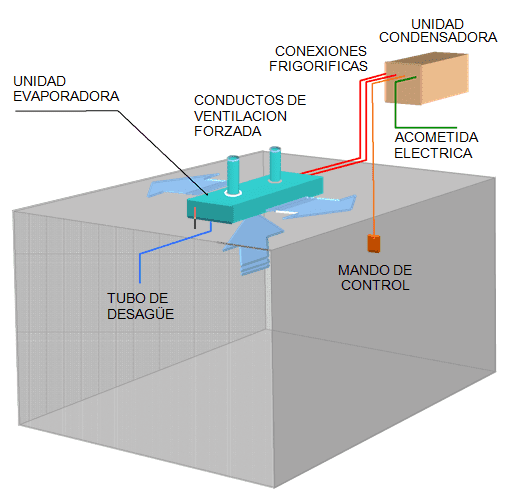
\includegraphics[width=0.45\textwidth]{figures/paredes-refri.png}
 	\caption{Vista general de la cámara de refrigeración} Fuente: \cite{intarcon-2023}
 	\label{fig:paredes-refri}
 \end{figure}
 
 En la figura \ref{fig:paredes-refri} las flechas indican el intercambio de calor producido por los componentes y el aire del sistemas
 
 
 \subsubsection{Cargas por infiltración de aire }
 
 El aire que entra en la cámara desde el exterior estará a una temperatura más alta que el aire que está en el interior. Por tanto, el sistema de refrigeración debe tener potencia suficiente para bajar la temperatura del aire de entrada hasta la temperatura de la cámara, vea la tabla \ref{tabla:renov-air} para tener una idea de cuántas veces en promediose renueva el aire en una cámara al día. Esa potencia se calculará con el producto del flujo másico de aire de renovación \( \dot{m}_{aire} \) (kg/s) por la diferencia de entalpías específicas en las condiciones correspondientes (\( h_{aire_{ext}} - h_{aire_{int}} \)) (kJ/kg).
 \begin{equation}
 	\dot{Q}_{aire} = \dot{m}_{aire} \cdot (h_{aire_{ext}} - h_{aire_{int}})
 \end{equation}
 La entalpía del aire será la suma de la correspondiente al aire seco y la del vapor de agua mezclado con el mismo:
 \begin{equation}\label{eq:entalp-air}
 	h_{aire \, húmedo} = h_{aire} + \omega_{aire} \cdot h_{vapor}
 \end{equation}
 La entalpía específica del aire a presión atmosférica se puede calcular como el producto del calor específico a esa presión por la temperatura (\( C_{p_{aire}} = 1.005 \, \text{kJ/kg} \, ^\circ \text{C} \)):
 \begin{equation}
 	h_{aire} = C_{p_{aire}} \cdot T_{aire}
 \end{equation}
 \begin{equation}
 	h_{aire} = 1.005 \cdot T \, \text{kJ/kg} \, ^\circ \text{C} 
 \end{equation}
 La entalpía del vapor por unidad de masa de aire seco se calcula como el producto de la humedad específica del aire (\( \omega_{aire} \)) por la suma del calor latente absorbido en el proceso de evaporación a presión atmosférica (\( \lambda = 2503 \, \text{kJ/kg} \, \text{agua} \)) y el calor específico a esa presión por la temperatura:
 \begin{equation}
 	h_{vapor} = \omega_{aire} \cdot (\lambda + C_{p_{vapor}} \cdot T)
 \end{equation}
 \begin{equation}
 	\lambda = 2503 \, \text{kJ/kg} \, \text{agua}
 \end{equation}
 \begin{equation}
 	C_{p_{vapor}} = 1.86 \, \text{kJ/kg} \, \text{agua}\, ^\circ \text{C} 
 \end{equation}
 De ahí se obtiene la Ecuación \ref{eq:entalp-air} por la que se puede calcular la entalpía del aire húmedo a partir de su temperatura y su humedad absoluta:
 \begin{equation}
 	h_{aire} = C_{p_{aire}} \cdot T + \omega_{aire} \cdot (\lambda + C_{p_{vapor}} \cdot T)
 \end{equation}
 Si se desea expresar la entalpía en relación al volumen de aire, se debe multiplicar por la densidad del mismo \( \rho \):
 \begin{equation}
 	hV_{aire} = (C_{p_{aire}} \cdot T_{vapor} + \omega_{aire} \cdot (\lambda + C_{p_{vapor}} \cdot T_{vapor})) \cdot \rho
 \end{equation}
 La densidad se  calcula con la ecuación:
 \begin{equation}
 	\rho = \frac{PM_{aire}}{R \cdot T}
 \end{equation}
 Donde: \( PM_{aire} \) es el peso molecular del aire (28.93 g/mol), \( T \) es la temperatura del aire en K, y \( R \) es la constante universal de los gases (0.082 litros Pa/mol K).\\
 Sabiendo el volumen que se renueva periódicamente en la cámara, se puede calcular el calor empleado en el enfriamiento del aire mediante la ecuación:
 \begin{equation}
 	\dot{Q}_{aire} = n \cdot V \cdot (hV_{aire_{ext}} - hV_{aire_{int}})
 \end{equation}

 
 \begin{table}[H]
 	\centering
 	\caption{Estimación del número de veces que se renueva el aire en las cámaras por día}\cite{Martin}
 	\begin{tabular}{cccccc}
 		\toprule
 		Renovaciones por día & Renovaciones por día & Volumen (m\textsuperscript{3}) & T <0ºC & T >0ºC & Volumen (m\textsuperscript{3}) \\
 		\midrule
 		2,5 & 52 & 70 & 100 & 6,8 & 9 \\
 		3 & 47 & 63 & 150 & 5,4 & 7 \\
 		4 & 40 & 53 & 200 & 4,6 & 6 \\
 		5 & 35 & 47 & 250 & 4,1 & 5,3 \\
 		7,5 & 28 & 38 & 300 & 3,7 & 4,8 \\
 		10 & 24 & 32 & 400 & 3,1 & 4,1 \\
 		15 & 19 & 26 & 500 & 2,8 & 3,6 \\
 		20 & 16,5 & 22 & 600 & 2,5 & 3,2 \\
 		25 & 14,5 & 19,5 & 800 & 2,1 & 2,8 \\
 		30 & 13 & 17,5 & 1000 & 1,9 & 2,4 \\
 		40 & 11,5 & 15 & 1500 & 1,5 & 1,95 \\
 		50 & 10 & 13 & 2000 & 1,3 & 1,65 \\
 		60 & 9 & 12 & 2500 & 1,1 & 1,45 \\
 		80 & 7 & 10 & 3000 & 1,05 & 1,05 \\
 		\bottomrule
 	\end{tabular} \label{tabla:renov-air}
 \end{table}
 \subsubsection{Cargas del producto a refrigerar}
 La carga térmica más importante en una cámara proviene de los productos que se pretenden refrigerar. El calor empleado en el proceso depende de la temperatura de entrada de los productos y la temperatura a la que se desea realizar la conservación en frío. Este calor se puede dividir en cuatro partes:
 \begin{enumerate}
 	\item Calor de enfriamiento por encima del punto de congelación:
 	
  
  \begin{equation}
 	\dot{Q}_{\text{enf1}} = \dot{m} \cdot C_e \cdot (T_e - T_{\text{cong}})
 	\label{eq:Calor-de-enfriamiento}
 \end{equation}
 \item Calor de congelación

 \begin{equation}
 	\dot{Q}_{\text{cog}} = \dot{m} \cdot L_{\text{cong}}
 \end{equation}
 
 El calor latente de congelación de un producto ($L_{\text{cong}}$) puede ser obtenido en la bibliografía p.ej \cite{bohn}, donde existen numerosas tablas para diferentes tipos de productos; o puede ser estimado a partir de su contenido de agua con la siguiente fórmula: $L_{\text{cong}} = 3{.}335 \cdot a$
 \item Calor de enfriamiento por debajo del punto de congelación
 \begin{equation}
 	\dot{Q}_{\text{enf2}} = \dot{m} \cdot C_{e\text{cong}} \cdot (T_{\text{cong}} - T_f)
 \end{equation}
 \item Calor de respiración del producto
 \begin{equation}
 	\dot{Q}_{\text{resp}} = \dot{m} \cdot L_{\text{resp}}
 \end{equation}
\end{enumerate}
 
 En \citeNP{Martin} se mencionan otras cargas que se podrían considerar como secundarias, pero no podemos excluirlas del cálculo son:
\begin{itemize}
	\item  Carga por radiación solar
	\item Carga por ocupación (personal laborando)
	\item Por iluminación
	\item  Por motores
	
\end{itemize}

\subsection{Sistema de refrigeración}
\subsubsection{Selección del evaporador}
Luego se continua con la elección del evaporador, para ello debemos conocer:
\begin{itemize}
	\item Temperatura Saturada de Succión \begin{equation}
		T_{sat.succ} = T_{camara} - 10^\circ F
	\end{equation}
	\item Temperatura Saturada de Evaporación \begin{equation}
		T_{sat.succ} =T_{sat.evap}
	\end{equation}	
\end{itemize}

\begin{figure}[H]
	\centering
	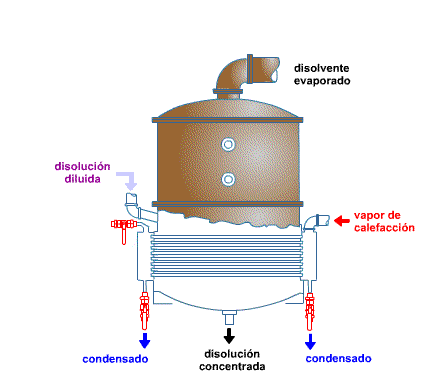
\includegraphics[width=0.5\linewidth]{figures/evap-func}
	\caption{Funcionamiento del evaporador}
	\label{fig:evap-func}
\end{figure}
\begin{figure}[H]
	\centering
	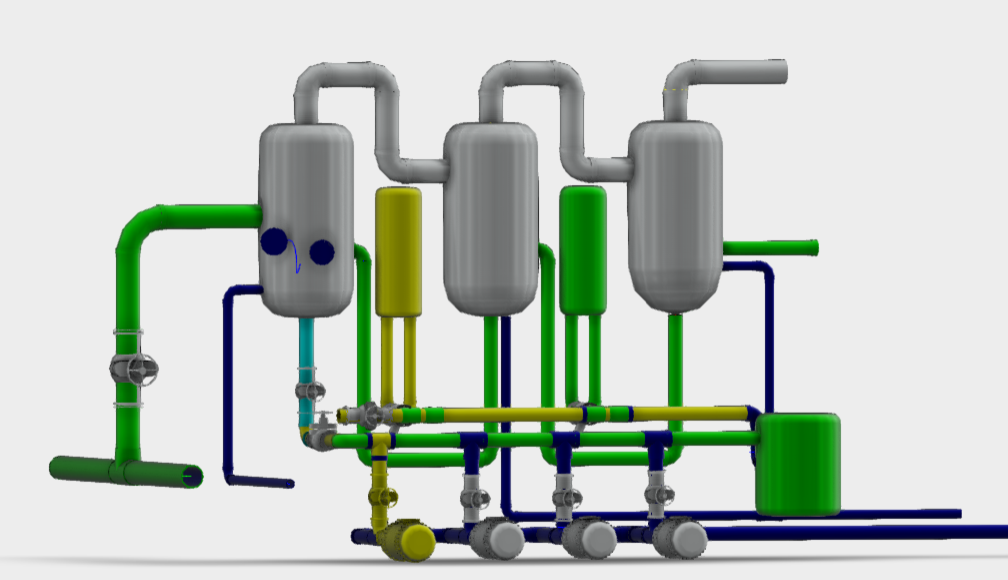
\includegraphics[width=0.576\linewidth]{figures/evap-cad1}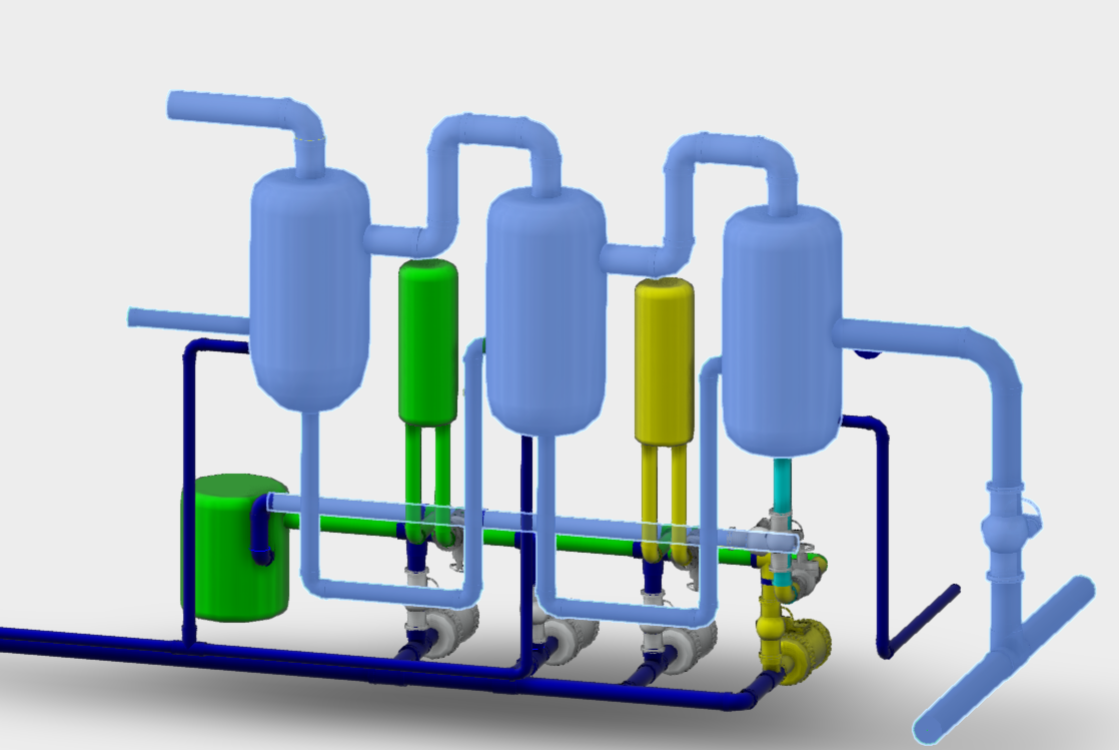
\includegraphics[width=0.5\linewidth]{figures/evap-cad2}
	\caption{Vistas de un sistema de evaporador. Creado en AutoCAD, basado en} \cite{bibliocad}
	\label{fig:evap-cad}
\end{figure}
 
 
 Con este dato, y el dato de los BTU de requerimiento de la carga térmica, se selecciona el evaporador más conveniente, también  considerando el diseño espacial de la cámara frigorífica, en donde podremos elegir  entre los siguientes tipos de evaporador, vea las figuras \ref{fig:evap-func} y \ref{fig:evap-cad}, para comprender los tipos de evaporador que se mencionan aquí:(a) Evaporadores perfil bajo; (b) Evaporadores perfil medio; (c) Evaporadores perfil alto; (d) Evaporadores perfil industrial y (e) Evaporadores de techo.
 
 \subsubsection{Selección de motor}
 
 Una vez seleccionado el evaporador y determinado el número de motores-ventilador, procedemos a calcular el calor que estos generan. Si no se conocen las cargas debidas a los motores, se pueden hacer las siguientes suposiciones:
 \begin{itemize}
 	\item Un motor de 1 HP por cada 16,000 ft\textsuperscript{3} en cámaras de refrigeración.\vspace*{-0.2cm}
 	\item Un motor de 1 HP por cada 12,500 ft\textsuperscript{3} en cámaras de congelación.
 \end{itemize}\vspace*{-0.2cm}
 La selección de un motor adecuado implica considerar varios factores para garantizar un rendimiento óptimo en una aplicación específica, como los requisitos de la aplicación, el tipo de motor, la eficiencia y el rendimiento. Esto se facilita mediante la tabla \ref{tabla:motores}.
 

 
 
 Entonces, para calcular el calor emitido por los motores del evaporador, usamos la fórmula:
 \begin{equation}\label{eq:emision_calor_motores}
 	Q_{EME} = \text{No. de Motores en HP} \times \text{Calor equivalente} \times 24
 \end{equation}
 Con esta carga recalculamos la carga térmica parcial agregándole este valor, para luego agregarle el factor de seguridad del 10\%, y al finalizar, multiplicarlo por el número de horas estimadas.
 
 Cuando se ha determinado la carga térmica total por hora, se puede seleccionar el equipo basado en la información obtenida del trabajo inicial de reconocimiento. Algunos otros factores que afectan la selección del equipo son:\vspace*{-0.2cm}
 \begin{itemize}
 	\item Balance del equipo\vspace*{-0.2cm}
 	\item Diferencial de temperatura del sistema (°DT)\vspace*{-0.2cm}
 	\item Control de la capacidad/seguridad del producto\vspace*{-0.2cm}
 	\item Tipo de operación/flujo del aire.
 \end{itemize}\vspace*{-0.2cm}
 Balance del equipo. La capacidad de la unidad condensadora debe ser seleccionada a una temperatura saturada de succión que esté balanceada con el evaporador(es) a un diferencial de temperatura entre el refrigerante en el evaporador y el aire en la cámara de almacenamiento refrigerado   \cite{intarcon-2023}.
  \begin{table}[H]
 	\centering
 	\caption{Selección de motores de acuerdo a su carga} Fuente: \cite{suarez-2022}\\
 	\begin{tabular}{ccccc}
 		\hline
 		HP      & Tipo de        & RPM     & Eficiencia a                    & BTU/hr \\
 		Nominal & motor          & Nominal & \multicolumn{1}{r}{Plena Carga} &        \\ \hline
 		0.5     & Polo Sombreado & 1500    & 35                              & 360    \\
 		0.08    &                &         &                                 & 580    \\
 		0.125   &                &         &                                 & 900    \\
 		0.16    &                &         &                                 & 1160   \\
 		0.25    & Fase dividida  & 1750    & 54                              & 1180   \\
 		0.33    &                &         & 56                              & 1500   \\
 		0.5     &                &         & 60                              & 2120   \\
 		0.75    & Tres fases     & 1750    & 72                              & 2650   \\ \hline
 	\end{tabular}\\
 	\label{tabla:motores}
 	Nota: Los evaporadores de bajo perfil ADT o BME usan motores EBM. El calor que emiten es equivalente a 273.73 BTU/hr
 \end{table}
\subsubsection{Bases teóricas de la refrigeración.}
\subsubsection{Energía.}
La energía $E$ es la capacidad para realizar trabajo. La energía de un sistema consta de energías internas $U$, cinéticas $K$ y potenciales $P$. La energía interna se compone de energías térmicas (sensible y latente), químicas y nucleares. A menos que haya una reacción química o nuclear, el cambio interno de un sistema se debe a un cambio en la energía térmica. El cambio total de energía de un sistema se expresa como:
\begin{equation}
	\Delta E = E_2 - E_1 = \Delta U + \Delta KE + \Delta PE
	\label{eq:energia_total}
\end{equation}
Para la mayoría de los casos, las energías cinética y potencial no cambian durante un proceso y el cambio de energía se debe al cambio en la energía interna:
\begin{equation}
	\Delta E = \Delta U = m(u_2 - u_1)
	\label{eq:energia_interna}
\end{equation}
La energía se mide en kJ o Btu (1 kJ = 0.94782 Btu). La energía por unidad de tiempo es la tasa de energía y se expresa como:
\begin{equation}
	\dot{E} = \frac{E}{t} \quad (\text{kW o Btu/h})
	\label{eq:energia_tasa}
\end{equation}
La unidad de la tasa de energía es kJ/s, que es equivalente a kW o Btu/h (1 kW = 3412.14 Btu/h). La energía por unidad de masa se llama energía específica; tiene la unidad de kJ/kg o Btu/lbm (1 kJ/kg = 0.430 Btu/lbm).
\begin{equation}
	e = \frac{E}{m} \quad (\text{kJ/kg o Btu/lbm})
	\label{eq:energia_especifica}
\end{equation}
La energía puede transferirse hacia o desde un sistema en tres formas: masa, calor y trabajo. Se describen brevemente en las siguientes secciones.

\subsubsection{Primera ley de la termodinámica}

Es bien sabido que la termodinámica es la ciencia de la energía y la entropía, y que la base de la termodinámica es la observación experimental. En la termodinámica, tales observaciones se formularon en cuatro leyes básicas de la termodinámica llamadas la cero, primera, segunda y tercera leyes de la termodinámica. Las primeras y segundas leyes de la termodinámica son las herramientas más comunes en la práctica, debido al hecho de que las transferencias y conversiones de energía están gobernadas por estas dos leyes, y en este capítulo nos enfocamos en estas dos leyes.

La primera ley de la termodinámica (PLT) se puede definir como la ley de la conservación de la energía, y establece que \textit{la energía no puede ser creada ni destruida}. Se puede expresar para un sistema general como el cambio neto en la energía total de un sistema durante un proceso es igual a la diferencia entre la energía total que entra y la energía total que sale del sistema:
\begin{equation}
	E_{\text{in}} - E_{\text{out}} = \Delta E_{\text{system}}
	\label{eq:primera_ley_energia}
\end{equation}
En forma de tasa,
\begin{equation}
	\dot{E}_{\text{in}} - \dot{E}_{\text{out}} = \Delta \dot{E}_{\text{system}}
	\label{eq:primera_ley_energia_tasa}
\end{equation}
Para un sistema cerrado que experimenta un proceso entre estados inicial y final que involucran interacciones de calor y trabajo con los alrededores (Figura \ref{fig:sistema_cerrado}),
\begin{equation}
	E_{\text{in}} - E_{\text{out}} = \Delta E_{\text{system}}
	\label{eq:primera_ley_energia_sistema_cerrado}
\end{equation}
$(Q_{\text{in}} + W_{\text{in}}) - (Q_{\text{out}} + W_{\text{out}}) = \Delta U + \Delta KE + \Delta PE$
\begin{figure}[H]
	\centering
	\begin{tikzpicture}
		% Dibujo del sistema cerrado
		\draw (0,0) rectangle (4,3) node[pos=.5] {System};
		
		% Etiquetas de los estados
		%	\node at (2,2.5) {Estado 1};
		%	\node at (2,0.5) {Estado 2};
		
		% Etiquetas de las interacciones
		\node at (-1,1.5) {$W_{in}$};
		\node at (5,1.5) {$W_{out}$};
		\node at (2,4) {$Q_{in}$};
		\node at (2,-1) {$Q_{out}$};
		
		
	\end{tikzpicture}
	\caption{Representación de un sistema cerrado con interacciones de calor $Q$ y Trabajo $W$ sin intercambio de masa.  }(Fuente: Propia, basado de \cite{james-2013}) 
	\label{fig:sistema_cerrado}
\end{figure}
Si no hay cambio en las energías cinética y potencial,
\begin{equation}
	(Q_{\text{in}} + W_{\text{in}}) - (Q_{\text{out}} + W_{\text{out}}) = \Delta U = m(u_2 - u_1)
	\label{eq:primera_ley_energia_sistema_cerrado_2}
\end{equation}
Consideremos un volumen de control que involucra un proceso de flujo estable. La masa está entrando y saliendo del sistema y hay interacciones de calor y trabajo con los alrededores (Figura \ref{fig:sistema_abierto}). Durante un proceso de flujo estable, el contenido total de energía del volumen de control permanece constante, y por lo tanto, el cambio total de energía del sistema es cero. Entonces, la PLT puede expresarse como:
\begin{equation}
	\dot{E}_{\text{in}} - \dot{E}_{\text{out}} = \Delta \dot{E}_{\text{system}} = 0
\end{equation}
\begin{equation}
	\dot{E}_{\text{in}} = \dot{E}_{\text{out}}
\end{equation}
\begin{equation}
	\dot{Q}_{\text{in}} + \dot{W}_{\text{in}} + \dot{m}h_{\text{in}} = \dot{Q}_{\text{out}} + \dot{W}_{\text{out}} + \dot{m}h_{\text{out}}
\end{equation}
Aquí, las energías cinética y potencial son despreciadas.


\begin{figure}[H]
	\centering
	\begin{tikzpicture}
			\tikzstyle{arrow} = [thick,->,>=stealth]
		\tikzstyle{line} = [draw, -latex']
		\draw (0,0) rectangle (4,3) node[pos=.5] {Sistema};
		
		% Etiquetas de las interacciones
		\node at (-1,1.5) {$W_{\text{in}}$};
		\node at (5,1.5) {$W_{\text{out}}$};
		\node at (2,4) {$Q_{\text{in}}$};
		\node at (2,-1) {$Q_{\text{out}}$};
		
		% Flechas de las interacciones s.abierto
		
		
			\path [line] (-0.5,1.5) -- (0.5,1.5);
			\path [line] (4.5,1.5) -- (3.5,1.5);
			\path [line](2,2) -- (2,2.9);
			\path [line] (2,0) -- (2,1);
		
		% Línea de cambio de masa
		%                       izq           derecha
			\path [line] (-3,2.5) -- (1,2);
		\path [line] (6,3) -- (3,2);
		
		% Etiqueta de cambio de masa
		\node at (-3,2.8) {$\dot{m}$};
		\node at (6,3.2) {$\dot{m}$};
	\end{tikzpicture}
	\caption{Representación de un sistema abierto con interacciones de calor $Q$ y Trabajo $W$. Los intercambios de masa son las líneas con la $\dot{m}$ fuera del sistema. }(Fuente: Elaboración propia, basado de \cite{james-2013})
	\label{fig:sistema_abierto}
\end{figure}

\subsubsection{Segunda ley de la termodinámica}
La mayoría de los procesos de refrigeración y bombas de calor operan de manera cíclica, devolviendo periódicamente el refrigerante a un estado dado. Por lo tanto, podemos decir que durante el ciclo el cambio neto en la energía interna es cero, es decir:
\begin{equation}
	0 = \Delta \int_{\text{cycle}} U \equiv \oint\Delta U = 0
\end{equation}
y por lo tanto, la primera ley para un proceso cerrado y cíclico puede escribirse como:
\begin{equation}
	W_\text{net }  = Q_\text{net } 
\end{equation}
En los ciclos de refrigeración y bomba de calor, el trabajo se realiza solo durante una etapa del ciclo, mientras que el calor se transfiere durante dos etapas, una a baja temperatura y otra a alta temperatura (las temperaturas son "altas" y "bajas" relativas entre sí, en lugar de términos absolutos). Por lo tanto, la forma más útil de la Primera Ley para analizar ciclos de refrigeración o bomba de calor es:
\begin{equation}
	   W =Q_H -Q_C
\end{equation}
donde $W$ es el trabajo realizado sobre el refrigerante, y los subíndices $H$ y $C$ se refieren a los procesos de transferencia de calor de temperatura alta (caliente) y baja (fría), respectivamente.


\subsubsection*{Afirmaciones de la Segunda Ley}

La Segunda Ley de la Termodinámica es quizás ligeramente más abstracta y difícil de entender que la Primera Ley. Parafraseando a Rudolf Clausius (1822 a 1888), la Segunda Ley establece que:
\begin{center}
		\textit{$"$Es imposible construir un dispositivo que opere de manera cíclica cuyo único propósito sea transferir calor de un depósito de temperatura baja a un depósito de temperatura alta.$"$}
\end{center}
A primera vista, esta afirmación podría sugerir que la refrigeración (que es un proceso que tiene el efecto neto de transferir calor de una temperatura baja a una temperatura alta) es una imposibilidad física; sobre este punto más adelante.

Para obtener una expresión matemática de la Segunda Ley, primero necesitamos recordar la definición de entropía (como se usa en la termodinámica clásica) cortesía de Clausius:
\begin{equation}
	  \Delta S =\int \frac{Q_{rev}}{T}  
\end{equation}

También, la Segunda Ley puede escribirse como:
\begin{equation}\label{eq:sec-law-system}
  \Delta S_{\text{universe}} = \Delta S_{\text{system}} - \Delta S_{\text{surrounding}} \geq 0	
\end{equation}

Podemos expresar verbalmente la Ecuació \ref{eq:sec-law-system} diciendo que para cualquier proceso, la entropía del universo solo puede aumentar, o en el caso límite (procesos reversibles) puede permanecer sin cambios. La Segunda Ley establece que la entropía del universo nunca puede disminuir. \cite{james-2013}


\subsubsection{Formalismo de Refrigeración}

Un refrigerador es un dispositivo utilizado para transferir calor de un medio de baja temperatura a uno de alta temperatura. Son dispositivos cíclicos. La Figura \ref{fig:ref-comp} muestra el esquema de un ciclo de refrigeración por compresión de vapor (el tipo más común). Un fluido de trabajo (llamado refrigerante) ingresa al compresor en estado de vapor y es comprimido a la presión del condensador. El refrigerante de alta temperatura se enfría en el condensador al rechazar calor a un medio de alta temperatura. El refrigerante ingresa al dispositivo de expansión en estado líquido. Se expande en el dispositivo de expansión y su presión y temperatura disminuyen. El refrigerante es una mezcla de vapor y líquido en la entrada del evaporador. Absorbe calor de un medio de baja temperatura a medida que fluye en el evaporador. \cite{boles-2010}\\
El ciclo se completa cuando el refrigerante sale del evaporador en estado de vapor y entra en el compresor. 
Un balance de energía para un ciclo de refrigeración, basado en la ecuación \ref{eq:primera_ley_energia} de la PLT, da como resultado:
\begin{equation}
	QH = QL + W \label{eq:energy_balance}
\end{equation}

El indicador de eficiencia para un ciclo de refrigeración es el coeficiente de rendimiento (COP), que se define como el calor absorbido del espacio enfriado dividido por el trabajo de entrada en el compresor:

\begin{equation}
	COP_R = \frac{QL}{W} \label{eq:COP_definition}
\end{equation}

Esto también se puede expresar como:

\begin{equation}
	COP_R = \frac{QL}{QH - QL} = \frac{1}{QH / QL - 1} \label{eq:COP_expression}
\end{equation}

\begin{figure}[H]
	\centering
	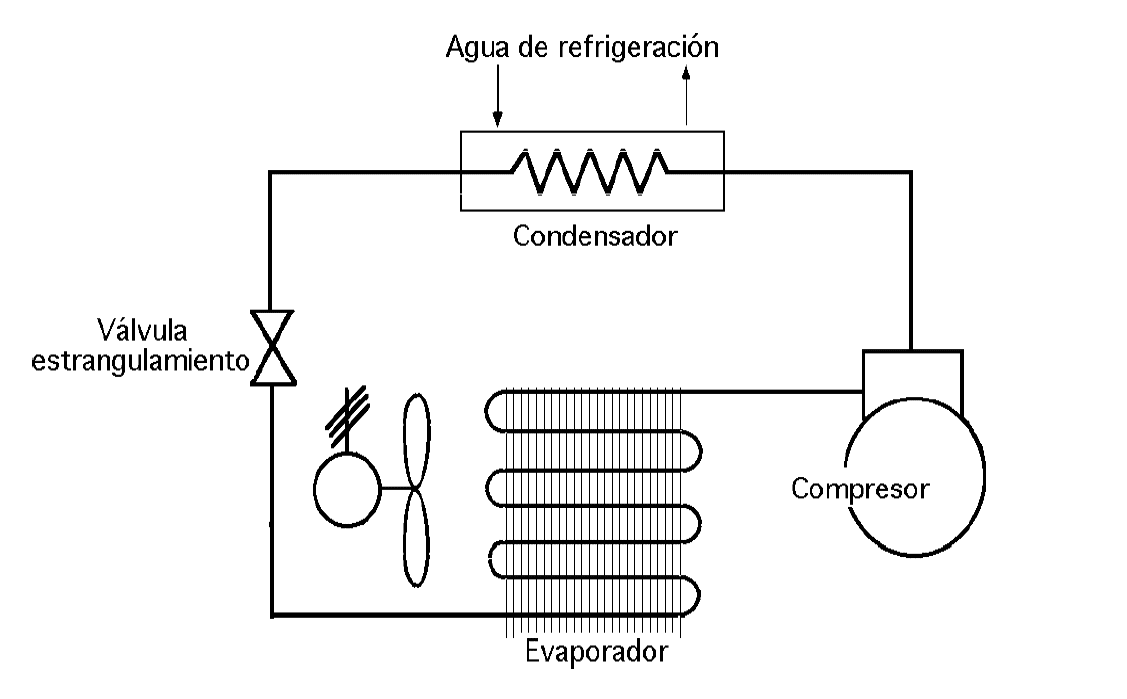
\includegraphics[width=0.7\textwidth]{figures/ref-comp.png}
	\caption{Diagrama esquemático del ciclo de refrigeración por compresión de vapor.} Fuente: \cite{theoms-2023}
	\label{fig:ref-comp}
\end{figure} 
\subsection{Distribución del Aire}
El diseño de sistemas HVAC a menudo se basa en decisiones predeterminadas, como suministrar agua fría a 5°C o aire acondicionado a 13°C, debido a su efectividad comprobada. Sin embargo, estas decisiones tienen implicaciones directas en los costos de tuberías, conductos y equipos, lo que afecta el gasto de capital y la comodidad \cite{hvac-2016}
\begin{itemize}
	\item Equipos de manejo de aire más pequeños reducen el gasto de capital y liberan espacio adicional debido a su huella más pequeña.
\item La distribución de aire frío puede ahorrar espacio significativo. Por ejemplo, un manejador de aire típico que necesita 34,485 pies cúbicos por minuto (cfm) para aire a 13°C solo requiere 20,900 cfm para aire a 7°C. Esto reduce el área frontal de la bobina y permite conductos más pequeños y sencillos.
\item| Conductos más pequeños significan menos chapa metálica, instalación más fácil y más espacio en el techo para bandejas de cables. Además, los conductos redondos permiten velocidades de aire más altas y reducen aún más el tamaño del conducto.
\item Una altura de piso a piso más corta, gracias a los conductos más pequeños, puede reducir los costos de vidrio y acero en edificios de varios pisos, e incluso agregar un piso de espacio alquilable.
\item Una menor potencia del ventilador reduce los costos de instalación eléctrica y operativos durante la vida útil del edificio, y puede disminuir el ruido del ventilador \cite{tecfrinor}.
\end{itemize}
El cálculo del flujo de aire se realiza multiplicando el área total de la habitación por la altura del techo y el número de cambios de aire por hora (ACH), y dividiendo todo entre 60 minutos para obtener los CFM (pies cúbicos por minuto) \cite{bercofred-2021}.

\begin{equation}
	 {CFM} = \frac{ {Área} \times  {Altura} \times  {ACH}}{60}
\end{equation}

En una cámara refrigerada estándar, la humedad relativa (HR) generalmente se mantiene entre el 90\% y el 100\%. Cuando la HR alcanza niveles del 90\% al 100\%, la formación de condensación es casi inevitable. La presencia no deseada de humedad en el aire crea un ambiente propicio para el crecimiento de contaminantes, lo que puede representar una amenaza para los productos almacenados.
\subsection{Dimensionamiento de puerta}

Las puertas desempeñan un papel importante en el equilibrio termodinámico de la cámara de refrigeración, ya que representan puntos de entrada y salida de aire que pueden afectar significativamente la eficiencia energética y la estabilidad térmica de la cámara. Especialmente en el caso de la refrigeración de insulina, donde se requiere un control preciso de la temperatura, las puertas deben diseñarse y ubicarse estratégicamente para minimizar la pérdida de frío y mantener un ambiente interno constante y seguro para el almacenamiento de medicamentos sensibles a la temperatura. Por lo tanto, elegir puertas adecuadas y gestionar su uso de manera eficiente es fundamental para garantizar un rendimiento óptimo del sistema de refrigeración y la integridad de los productos almacenados. 
 
 
 

\section{Lineamientos de regulación del sistema artefactual (Normativas y regulaciones)}

Las Normas Oficiales Mexicanas (NOM) son leyes técnicas de obligado cumplimiento emitidas por las autoridades competentes, cuyo objetivo es establecer las condiciones que deben cumplirse si un proceso o servicio representa un riesgo para la seguridad humana, o pone en peligro la salud humana. También contiene información sobre los términos y referencias para el cumplimiento y aplicación de estos términos \cite{salud-2022}.
\subsection{Normas oficiales Mexicanas}
\begin{itemize}
	\item NOM-12-ENER-2019, Eficiencia energética de unidades condensadoras y evaporadoras para refrigeración. Límites, métodos de prueba y etiquetado.
	\item NOM-008-SCFI-2002, Sistema General de Unidades de Medida.
	\item NOM-197-SSA1-2000, Que establece los requisitos mínimos de infraestructura y equipamiento de hospitales y consultorios de atención médica especializada.
	\item NOM-028-STPS-2012, Sistema para la administración del trabajo-Seguridad en los procesos y equipos críticos que manejen sustancias químicas peligrosas.
	\item NOM-025-STPS-2008, Condiciones de iluminación en los
	centros de trabajo. Esta norma establece los requisitos para la iluminación en los
	centros de trabajo, con el fin de garantizar la seguridad y salud de los trabajadores.
\end{itemize}
Para mayor detalles del contexto normativo revise la \hyperref[sec:contexto-normativo]{sección 2.2}.
De acuerdo a la NOM-025-STPS-2008 se establecen los siguientes requisitos:


\begin{itemize}
	\item La iluminación debe ser suficiente para permitir a los trabajadores realizar sus actividades sin riesgos.
	\item Se requiere que la iluminación sea uniforme y sin deslumbramientos.
	\item La iluminación debe adaptarse adecuadamente al tipo de actividad que se realiza en el centro de trabajo.
\end{itemize}

\subsection{Recomendaciones para Cámaras Frigoríficas}

Además de cumplir con los requisitos normativos, se sugieren las siguientes recomendaciones para garantizar una iluminación adecuada en cámaras frigoríficas:

\begin{itemize}
	\item Emplear luminarias altamente eficientes en términos energéticos.
	\item Ajustar la altura de las luminarias para lograr una distribución uniforme de la luz.
	\item Seleccionar luminarias con un ángulo de apertura apropiado para el área que se va a iluminar.
\end{itemize}

\subsection{Consideraciones Específicas para Cámaras Frigoríficas}

Al diseñar e instalar el sistema de iluminación en cámaras frigoríficas, se deben tener en cuenta consideraciones específicas:

\begin{itemize}
	\item La temperatura dentro de la cámara puede afectar el rendimiento de las luminarias, por lo que es crucial seleccionar aquellas diseñadas para funcionar en entornos fríos.
	\item La humedad también puede influir en el rendimiento de las luminarias, por lo que se deben elegir luminarias resistentes a la humedad.
	\item La condensación es un problema potencial en estas cámaras, por lo que se deben seleccionar luminarias diseñadas para prevenir la acumulación de humedad.
\end{itemize}

\subsection{Normativa y requisitos para cámaras frigoríficas comerciales}

La Norma Oficial Mexicana NOM-001-SCFI-2018 establece requisitos de seguridad y métodos de prueba para aparatos electrónicos, incluyendo cámaras frigoríficas comerciales. Esta norma incluye los siguientes requisitos específicos:

\begin{itemize}
	\item \textbf{Protección contra Riesgos Eléctricos:} Se requiere un interruptor diferencial de alta sensibilidad para proteger los circuitos eléctricos, y los aparatos deben conectarse a tomas de corriente con conexión a tierra.
	\item \textbf{Protección contra Riesgos Mecánicos:} Las puertas y ventanas deben estar diseñadas para prevenir atrapamientos y lesiones, y deben contar con sistemas de cierre seguro.
	\item \textbf{Protección contra Riesgos Térmicos:} Se exige un adecuado sistema de aislamiento térmico para evitar quemaduras y exposición a temperaturas extremas.
	\item \textbf{Protección contra Riesgos de Incendio:} Se requiere un sistema de alarma de fugas de refrigerante y un sistema de extinción de incendios adecuado.
	\item \textbf{Seguridad de Puertas:} Las puertas deben poder abrirse desde el interior sin necesidad de llave, incluso si tienen cerraduras externas. En temperaturas bajo cero, se deben instalar dispositivos de calentamiento para evitar la congelación de las puertas.
\end{itemize}
\section{Conceptualización De Sistema Artefactual (bosquejo general)}
El diseño inicial del equipo a diseñar representará de forma muy simplificada las ideas subyacentes deñ diseño. Para el diseño preliminarse hará uso de Inventor 2025 siguiendo alguno de estos pasos.
\begin{enumerate}
	\item \textbf{Definir Dimensiones:} Establecer las dimensiones generales hipotéticas de la cámara de refrigeración, incluyendo altura, anchura y profundidad.
	\item \textbf{Diseñar Paredes Aisladas:} Utilizar las herramientas de modelado para diseñar las paredes aisladas de la cámara, asegurándose de considerar el material aislante adecuado.
	\item \textbf{Ubicar Unidades de Refrigeración:} Colocar las unidades de refrigeración dentro del espacio de la cámara, asegurándose de dejar suficiente espacio para la circulación del aire.
	\item \textbf{Agregar Puntos de Acceso:} Incluir en el diseño posibles puntos de acceso, como puertas o paneles desmontables, asegurándose de que estén ubicados estratégicamente para facilitar el acceso al interior de la cámara.
	\item \textbf{Revisión y Ajustes:} Revisar el bosquejo preliminar para asegurarse de que cumple con los requisitos y especificaciones del diseño.
\end{enumerate}

El bosquejo preliminar (ver figura \ref{fig:design1}) proporciona una representación inicial de la disposición y estructura general de la cámara de refrigeración, permitiendo visualizar y comunicar conceptos antes de avanzar hacia diseños más detallados y completos. Este proceso creativo es fundamental para desarrollar una solución efectiva y funcional para la refrigeración de insulina.



\subsection{Bosquejo general del sistema: cámara frigorífica}\rsp
\begin{figure}[H]
	\centering
	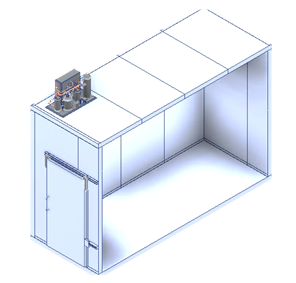
\includegraphics[width=0.6\linewidth]{figures/design-cooler2}
	\caption{Vista frotal 3D de la cámara vacía y sus componentes escenciales}
	\label{fig:design1}
\end{figure}
\begin{figure}[H]
	\centering
	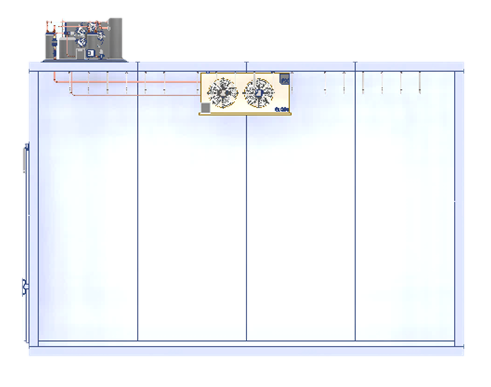
\includegraphics[width=0.6\linewidth]{figures/design-latder}
	\caption{Vista lateral derecha  de la cámara y sus componentes de enfriamiento}
	\label{fig:design-latder}
\end{figure}
La figura \ref{fig:design1} muestra el diseño desde un panorama completo y sus componenentes esenciales, así mismo se muestra el espacio dentro de la cámara.
Mientras que en la figura \ref{fig:design-latder} se muestra una vista en donde puede apreciarse el sistema de enfriamiento y el sistema de tubos dentro de la cámara, más adelante se proporcionarán vistas específico.


\subsection{Diagrama a bloques del proceso de trabajo}

Los diagramas de bloques o de flujo son herramientas visuales que permiten representar de manera clara y concisa el flujo de un proceso o sistema, así como las interacciones entre sus diferentes componentes. \cite{lucidchart-2022}\\
\textbf{Importancia de los diagramas de bloques o de flujo:}
\begin{itemize}
	\item Claridad y comprensión.
	\item Identificación de problemas.
	\item Diseño y planificación.
	\item Documentación y estandarización.
	\item Toma de decisiones.
\end{itemize}
Vea la figura \ref{fig:flujo_insulina} a \ref{fig:diagrama-procesos} para tener más detalles del proceso que se seguirá y de las condiciones que se tomarán en cuenta.

\subsubsection{Diagrama de flujo}

\begin{figure}[H]
	\centering
	\begin{tikzpicture}[node distance=2cm]
		\tikzstyle{startstop} = [ellipse, minimum width=3cm, minimum height=1cm, text centered, draw=black, fill=blue!10]
		\tikzstyle{process} = [rectangle, minimum width=3cm, minimum height=1cm, text centered, draw=black, fill=green!10]
		\tikzstyle{decision} = [diamond, minimum width=3cm, minimum height=1cm, text centered, draw=black, fill=red!10]
		\tikzstyle{arrow} = [thick,->,>=stealth]
		\tikzstyle{line} = [draw, -latex']
		\node (start) [startstop] {Inicio};
		\node (reception) [process, below of=start] {Recepción de insulina};
		\node (storage) [process, below of=reception] {Almacenamiento en UMF40};
		\node (distribution) [process, below of=storage] {Distribución y reordenamiento};
		\node (decision) [decision, below of=distribution, yshift=-1.5cm] {¿Cámara llena?};
		\node (inventory) [process, right of=decision, xshift=3cm] {Realizar inventario};
 
		\path [line] (start) -- (reception);
		\path [line] (reception) -- (storage);
		\path [line] (storage) -- (distribution);
		\path [line] (distribution) -- (decision);
		\path [line] (decision) -- node[anchor=south] {Sí} (inventory);
		\path [line] (decision.west) -- ++(-1,0) |- node[anchor=south east] {No} (reception);
		
	\end{tikzpicture}
	\caption{Diagrama de flujo para el proceso de gestión de insulina en una cámara frigorífica.}  Fuente: Elaboración propia, basado y hecho desde Tikz de \LaTeX \cite{Tan12}.
	\label{fig:flujo_insulina}
\end{figure}
 

 
\begin{figure}[H]
	\centering
	\begin{tikzpicture}[node distance=2cm]
		\tikzstyle{startstop} = [ellipse, minimum width=3cm, minimum height=1cm, text centered, draw=black, fill=blue!10]
		\tikzstyle{process} = [rectangle, minimum width=3cm, minimum height=1cm, text centered, draw=black, fill=green!10]
		\tikzstyle{decision} = [diamond, minimum width=3cm, minimum height=1cm, text centered, draw=black, fill=red!10]
	%	\tikzstyle{arrow} = [thick,->,>=stealth]
		\tikzstyle{line} = [draw, -latex']
		
		\node (start) [startstop] {Inicio};
		\node (precooling) [process, below of=start] {Pre-enfriamiento};
		\node (efficiency) [process, below of=precooling] {Evitar pérdida de eficiencia};
		\node (coldstorage) [process, below of=efficiency] {Almacenamiento en frío};
		\node (control) [process, below of=coldstorage] {Control de variables};
		\node (monitoring) [process, below of=control] {Sistema de monitoreo};
		\node (decision1) [decision, below of=monitoring, yshift=-1.5cm] {¿Se mantiene la eficacia?};
		\node (highdemand) [decision, below left of=decision1, xshift=-2.5cm, yshift=-2.5cm] {¿Hay alta demanda?};
		\node (distribute) [process, below of=highdemand, yshift=-2cm] {Se distribuye el medicamento};
		\node (removal) [process, below right of=decision1, xshift=2.5cm, yshift=-2.5cm] {Se retira el producto};
		\node (end) [startstop, below of=removal] {Fin};
		
		\path [line] (start) -- (precooling);
		\path [line] (precooling) -- (efficiency);
		\path [line] (efficiency) -- (coldstorage);
		\path [line] (coldstorage) -- (control);
		\path [line] (control) -- (monitoring);
		\path [line] (monitoring) -- (decision1);
		\path [line] (decision1.west) -| node[anchor=south east] {Sí} (highdemand);
		\path [line] (decision1.east) -| node[anchor=south west] {No} (removal);
		\path [line] (highdemand) -- node[anchor=east] {Sí} (distribute);
		\path [line] (highdemand.west) -- ++(-1,0) |- node[anchor=south east] {No} (start);
		\path [line] (removal) -- (end);
		
	\end{tikzpicture}
	\caption{Diagrama de flujo para el proceso de gestión de insulina en una cámara frigorífica.} Fuente: Elaboración propia, basado y hecho desde Tikz de \LaTeX  \cite{Tan12}. 
	\label{fig:flujo_ref-insu}
\end{figure}
 


\subsection{Diagrama de funcionamiento general de sistema}


\begin{figure}[H]
	\centering
	\begin{tikzpicture}[mindmap, grow cyclic, every node/.style={concept, font=\small,  }, level 1/.append style={sibling angle=90, font = \small, font=\bfseries}, level 2/.append style={sibling angle=60}]
		\node[concept, text=white, font=\bfseries]{Diseñar una cámara de refrigeración para conservar insulina en la CDMX}
		child [concept color=red!30] {
			node {Conservar la eficiencia de la insulina}
			child [concept color=green!20, level distance=4cm] { node {Medicamentos de calidad} }
			child [concept color=green!20, level distance=4cm] { 
				node {Evitar pérdidas de producto}
				child [concept color=yellow!30, level distance=4cm, font= \small] { node {Controlar pérdidas por temperaturas altas} }
			}
		}
		child [concept color=blue!30] {
			node {Apoyar a pacientes diabéticos}
			child [concept color=orange!30, level distance=4cm] { 
				node {Impulsar la calidad en medicamentos de UMF 40}
				child [concept color=violet!30, level distance=4cm] { node {Inocuidad pública de calidad} }
			}
			child [concept color=orange!30, level distance=4cm] { 
				node {Reducir las tasas de mortalidad por la diabetes}
				child [concept color=violet!30, level distance=4cm] { node {Tratamientos seguros} }
				child [concept color=violet!30, level distance=4cm, font = \tiny] { node {Control de la degradación de la insulina} }
			}
			child [concept color=orange!30, level distance=4cm] { node {Apoyar en aforo de pacientes a UMF cercanas} }
		};
	\end{tikzpicture}
	\caption{Mapa mental para el diseño de una cámara de refrigeración para conservar insulina en la CDMX.}
	\label{fig:diagrama-procesos} Fuente: Elaboración propia, basado y hecho desde Tikz de \LaTeX \cite{Tan12}.
\end{figure}
  
\section{Listado de partes de los componentes del sistema}
 
En la figura \ref{fig:design1} se muestran los componentes principales a trabajar y se enumeran de  la siguiente forma:
\begin{enumerate}
	\item  Paneles superiores: elementos que formarán parte del techo de la cámara. (Ver figura \ref{fig:design1})
	\item  Paneles laterales: elementos que funcionarán como paredes y contendrán la
	temperatura en condiciones óptimas. (Ver figuras \ref{fig:design1} y \ref{fig:design-latder})
	\item  Accesos: Puertas/ventanas: permitirán el control y distribución del aire dentro (Ver figura \ref{fig:design-front} )
	y fuera de la cámara frigorífica.
	\item  Equipo de enfriamiento: elemento encargado de proporcionar frio y 
	transmitirlo al interior del recinto frigorífico. (Ver figuras \ref{fig:design-enfria} y \ref{fig:design-ventils})
	\item  Recubrimiento lateral: Material que recubre las paredes; estos ayudarán a 
	aislar y conservar la temperatura del recinto.
	\item  Recubrimiento superior: Material que recubre el techo; estos ayudarán a 
	aislar y conservar la temperatura del recinto.
\end{enumerate}
En la siguiente figura (\ref{fig:design-front}) podemos apreciar la vista frontal de la cámara en donde se contará con una puerta corrediza, con las consideraciones ya descritas con anterioridad.
 
 \begin{figure}[H]
	\centering
	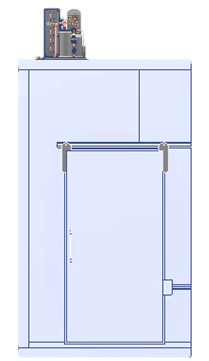
\includegraphics[width=0.3125\linewidth]{figures/design-front}
	\caption{Vista frontal de la cámara.} Fuente: Elaboración propia basado de \citeNP{bibliocad}
	\label{fig:design-front}
\end{figure}



\newcolumntype{J}{>{\raggedright\arraybackslash}p{10cm}}


\newpage 


\section{Identificación del conjunto y/o subconjunto por área tecnológica} %3.9
\textit{¿Cómo se relacionan entre sí los elementos componentes?}\\
De la sección anterior (3.8) se tiene la siguiente lista de componentes principales del sistema de refrigeración a diseñar, los cuales son señalados en la figura \ref{fig:listacomponentes} y descritos en la tabla \ref{tabla:lista-componentes}

\begin{figure}[H]
	\centering
	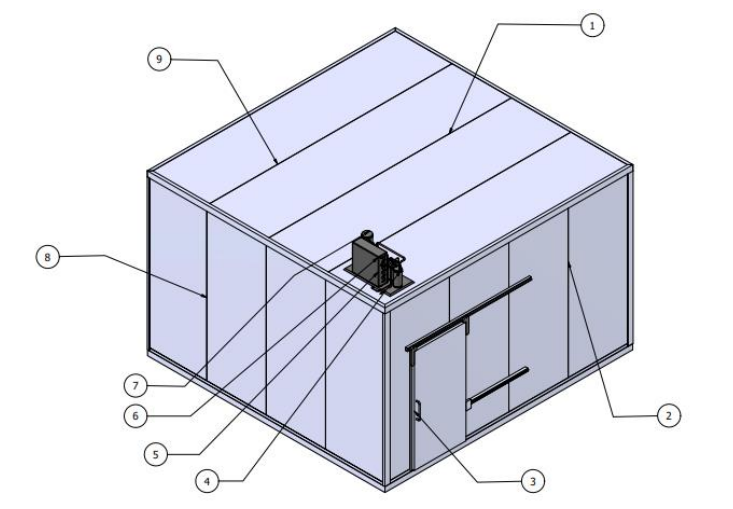
\includegraphics[width=0.6\linewidth]{figures/lista_componentes}
	\caption{Elementos componentes principales del sistema de refrigeración a diseñar.}Fuente: Elaboración propia basado de \citeNP{bibliocad}
	\label{fig:listacomponentes}
\end{figure}

\begin{table}[H]
	\centering
	\caption{Identificación de elementos principales de forma general del sistema.}
	\begin{tabular}{@{}cl@{}}
		\toprule
		\textbf{Número}           & \textbf{Nombre del elemento o componente}           \\
		\midrule
		1                         & Paneles superiores (techo)                          \\
		2                         & Paneles laterales (paredes)                         \\
		3                         & Puertas/ventanas                                    \\
		4                         & evaporador                                          \\
		5                         & condensador                                         \\
		6                         & compresor                                           \\
		7                         & Válvula de expansión                                \\
		8                         & Recubrimiento lateral                               \\
		9                         & Recubrimiento superior                              \\ \bottomrule
	\end{tabular}
	\label{tabla:lista-componentes}
\end{table}

Como se ha descrito en capítulos previos, las cámaras de refrigeración son fundamentales en la cadena de frío, especialmente para productos sensibles como la insulina, que requiere condiciones específicas de almacenamiento para mantener su eficacia y seguridad. Conocer los elementos de una cámara de refrigeración por área tecnológica es crucial para asegurar que estos medicamentos se conserven adecuadamente. A continuación, se detallan las áreas tecnológicas y la importancia de cada una en el contexto del almacenamiento de insulina.
\newpage

La \cite{UG2022}, describe a través de su blog (un documento en extenso) los componentes de un sistema de refrigeración tradicional los cuales han sido adaptados para el sistema del presente proyecto, se detallan en las tablas de \ref{tabla:mecanicos} a \ref{tabla:ergonomia}.



\begin{table}[H]
	\centering
	\caption{Conjunto 1: Listado de componentes mecánicos/térmicos del sistema de refrigeración}
	Fuente: Elaboración propia basado de la \citeNP{UG2022}.
	\begin{tabular}{@{}cl@{}}
		\toprule
		%\textbf{Número} & 
		\begin{minipage}[t]{0.25\linewidth}\textbf{Nombre del elemento o componente}\end{minipage} & \begin{minipage}[t]{0.7\linewidth}\textbf{Descripción del conjunto o integración de subsistema}\end{minipage} \\
		
		\midrule
		%	1               &
		Compresor                                 & \begin{minipage}[t]{0.7\linewidth}El compresor es el corazón del sistema de refrigeración, esencial para mantener el refrigerante en movimiento.\end{minipage} \\
		%	2               &
		Evaporador                                & \begin{minipage}[t]{0.7\linewidth}Absorbe el calor del interior de la cámara, enfriando el aire para mantener una temperatura adecuada.\end{minipage} \\
		%	3               & 
		Condensador                               & \begin{minipage}[t]{0.7\linewidth}Disipa el calor del refrigerante al exterior, ayudando a mantener una temperatura constante en la cámara.\end{minipage} \\
		%	4               & 
		Ventiladores                              & \begin{minipage}[t]{0.7\linewidth}Aseguran la circulación de aire uniforme dentro de la cámara de refrigeración, evitando zonas de diferentes temperaturas.\end{minipage} \\
		%5               &
		Puertas y sellos                          & \begin{minipage}[t]{0.7\linewidth}Mantienen la integridad de la cámara, evitando la entrada de aire caliente y humedad.\end{minipage} \\
		
		Recubrimiento térmico              
		
		
		& \begin{minipage}[t]{0.7\linewidth}
			Contiene la temperatura  	dentro de la cámara 		  	frigorífica evitando perdidas 		  	de calor (paredes laterales y superiores).
		\end{minipage} \\
		
		
		\bottomrule
	\end{tabular}
	\label{tabla:mecanicos}
	
\end{table}


\begin{table}[H]
	\centering
	\caption{Conjunto 2: Listado de componentes eléctricos y electrónicos del sistema de refrigeración}
	Fuente: Elaboración propia basado de \citeNP{UG2022}.
	\begin{tabular}{@{}cl@{}}
		\toprule
		%	\textbf{Número} &
		\begin{minipage}[t]{0.25\linewidth}\textbf{Nombre del elemento o componente}\end{minipage} & \begin{minipage}[t]{0.50\linewidth}\textbf{Descripción del conjunto o integración de subsistema}\end{minipage} \\
		
		\midrule
		%	1               & 
		Termostato                                & \begin{minipage}[t]{0.5\linewidth}Controla y monitoriza la temperatura interna de la cámara, asegurando condiciones óptimas.\end{minipage} \\
		%2               &
		Sensores de temperatura                   & \begin{minipage}[t]{0.5\linewidth}Proporcionan lecturas precisas de la temperatura, fundamentales para el control del sistema.\end{minipage} \\
		%	3               & 
		Fuente de alimentación ininterrumpida & \begin{minipage}[t]{0.5\linewidth}Garantiza el funcionamiento continuo durante cortes de energía, evitando fluctuaciones de temperatura.\end{minipage} \\
		%4               &
		Generador de respaldo                     & \begin{minipage}[t]{0.5\linewidth}Proporciona energía durante apagones prolongados, asegurando el correcto funcionamiento del sistema.\end{minipage} \\ \bottomrule
	\end{tabular}
	\label{tabla:electricos}
\end{table}

\begin{table}[H]
	\centering
	\caption{Conjunto 3: Listado de componentes de automatización del sistema de refrigeración}
	Fuente: Elaboración propia basado de \citeNP{UG2022}.
	\begin{tabular}{@{}cl@{}}
		\toprule
		%\textbf{Número} & 
		\begin{minipage}[t]{0.25\linewidth}\textbf{Nombre del elemento o componente}\end{minipage} & \begin{minipage}[t]{0.60\linewidth}\textbf{Descripción del conjunto o integración de subsistema}\end{minipage} \\
		
		\midrule
		%	1               & 
		Controlador electrónico                   & \begin{minipage}[t]{0.6\linewidth}Regula el funcionamiento del sistema de refrigeración basado en lecturas de los sensores.\end{minipage} \\
		%	2               & 
		Sistema de monitoreo remoto               & \begin{minipage}[t]{0.6\linewidth}Permite la supervisión del sistema de refrigeración a distancia, facilitando la gestión y el mantenimiento.\end{minipage} \\
		%	3               & 
		Grabador de datos históricos              & \begin{minipage}[t]{0.6\linewidth}Registra las condiciones de temperatura a lo largo del tiempo, ayudando a mantener un registro detallado.\end{minipage} \\
		%4               &
		Sistemas de alarma                        & \begin{minipage}[t]{0.6\linewidth}Alertan sobre cualquier desviación de la temperatura, permitiendo acciones correctivas rápidas.\end{minipage} \\ \bottomrule
	\end{tabular}
	\label{tabla:automatizacion}
\end{table}




\begin{table}[H]
	\centering
	\caption{Conjunto 4: Listado de componentes ergonómicos del sistema de refrigeración}
	Fuente: Elaboración propia basado de \citeNP{UG2022}.
	\begin{tabular}{@{}cl@{}}
		\toprule
		%	\textbf{Número} &
		\begin{minipage}[t]{0.25\linewidth}\textbf{Nombre del elemento o componente}\end{minipage} & \begin{minipage}[t]{0.60\linewidth}\textbf{Descripción del conjunto o integración de subsistema}\end{minipage} \\ \midrule
		%	1               &
		Puertas de fácil acceso                   & \begin{minipage}[t]{0.6\linewidth}Diseñadas para un acceso sencillo y seguro a la cámara.\end{minipage} \\
		%2               &
		Panel de control intuitivo                & \begin{minipage}[t]{0.6\linewidth}Facilita la operación del sistema, con interfaces fáciles de entender y manejar.\end{minipage} \\
		%	3               &
		Iluminación interior adecuada             & \begin{minipage}[t]{0.6\linewidth}Proporciona una visibilidad clara dentro de la cámara, mejorando la seguridad y la eficiencia operativa.\end{minipage} \\
		%4               & 
		Racks ajustables                          & \begin{minipage}[t]{0.6\linewidth}Permiten la organización flexible del espacio de almacenamiento, optimizando el uso del espacio disponible.\end{minipage} \\ \bottomrule
	\end{tabular}
	\label{tabla:ergonomia}
\end{table}





\newpage
\section{Descripción de la interacción del elemento componente del sistema.}

Teniendo en cuenta que para la interacción entre elementos componentes debe existir algún tipo de movimiento, ya sea por transmisión o de transformación, los cuales en un equipo de refrigeración son poco comunes, entonces, para este apartado no se describirá una lista de componentes con este enfoque.



\section{Proceso del meta diseño de un sistema artefactual tecnológico}

\textit{Para que el producto tecnológico cumpla adecuadamente su función, ¿qué partes son esenciales y cuáles no?}\\


Se explica a continuación de acuerdo al autor \cite{de-leon-no-date} para que una cámara de refrigeración cumpla adecuadamente su función de almacenar y conservar la insulina, es vital realizar un meta diseño detallado. Este análisis permite identificar los componentes esenciales que aseguran el correcto funcionamiento del sistema de refrigeración y cuáles podrían ser prescindibles o de menor prioridad. Los componentes esenciales incluyen aquellos que directamente afectan la capacidad de mantener la temperatura adecuada, la seguridad y la estabilidad operativa del sistema.

\textbf{Importancia del metadiseño}
\begin{itemize}
	\item Optimización del funcionamiento: Al entender la función de cada componente, se pueden optimizar sus características y ubicaciones para mejorar el rendimiento del sistema.
	\item Eficiencia energética: Identificar componentes clave ayuda a mejorar la eficiencia energética del sistema, reduciendo costos operativos.
	\item Fiabilidad y durabilidad: Asegurar que los componentes esenciales sean de alta calidad aumenta la fiabilidad y durabilidad del sistema.
	\item Costos de mantenimiento: Identificar partes no esenciales permite reducir costos de mantenimiento y reparación, enfocándose en componentes críticos.
	\item Seguridad y cumplimiento: Un estudio detallado asegura que el sistema cumpla con las normas de seguridad y regulaciones pertinentes.
	
\end{itemize}


\textbf{Partes esenciales y no esenciales:}
\begin{itemize}
	\item Partes esenciales: Son aquellas cuyo fallo impactaría directamente en el funcionamiento de la cámara de refrigeración, como el compresor, el evaporador y los ventiladores.
	
	\item Partes no esenciales: Son componentes que, aunque necesarios, su fallo no detendría el sistema completo, como ciertos tornillos, pernos o elementos de soporte.
\end{itemize}

\newpage

\begin{landscape}
	En la tabla \ref{tabla:esenciales} se retoma la información y características principales de los elementos del sistema
	artefactual para su correcta función.
	
	
	\begin{table}[H]
		\centering
		\caption{Identificación de las partes esenciales de los componentes del sistema}
		Fuente: Elaboración propia basado de \cite{bohn}
		\begin{tabular}{@{}ccccccccc@{}}
			\toprule
			\textbf{Número} & \textbf{Componente}                                                              & \textbf{Duradero} & \textbf{Cambiable o} & \textbf{Flexible}    & \textbf{Comercial} & \textbf{Comercial}     & \multicolumn{2}{c}{\textbf{Selección}} \\  
			\textbf{}       & \textbf{}                                                                        & \textbf{}         & \textbf{modular}     & \textbf{o compuesto} & \textbf{nacional}  & \textbf{internacional} & \textbf{Sí}        & \textbf{No}       \\
			\midrule
			1               & \begin{tabular}[c]{@{}c@{}}Paneles \\ superiores\\ (techo)\end{tabular}          & 15 años           & cambiable            & flexible             & x                  &                        & x                  &                   \\
			2               & \begin{tabular}[c]{@{}c@{}}Paneles\\ laterales\\ (paredes)\end{tabular}          & 15 años           & cambiable            & flexible             & x                  &                        & x                  &                   \\
			3               & \begin{tabular}[c]{@{}c@{}}Puertas y \\ ventanas\end{tabular}                    & 15 años           & cambiable            & flexible             & x                  &                        & x                  &                   \\
			4               & Evaporador                                                                       & 10-12 años        & modular              & compuesto            & x                  & x                      & x                  &                   \\
			5               & Condensador                                                                      & 10-12 años        & modular              & compuesto            & x                  & x                      & x                  &                   \\
			6               & Compresor                                                                        & 10-12 años        & modular              & compuesto            & x                  & x                      & x                  &                   \\
			7               & \begin{tabular}[c]{@{}c@{}}Válvula\\ de expansión\end{tabular}                   & 10-12 años        & modular              & compuesto            & x                  & x                      & x                  &                   \\
			8               & \begin{tabular}[c]{@{}c@{}}Recubrimientos\\ (lateral y \\ superior)\end{tabular} & 15 años           & cambiable            & flexible             & x                  &                        & x                  &                   \\ \bottomrule
		\end{tabular}
		\label{tabla:esenciales}
	\end{table}
\end{landscape}
\newpage
\section{Alternativas tecnológicas de los componentes}
Evaluar alternativas tecnológicas para los componentes del sistema de refrigeración, planteando los requerimientos técnicos y mostrando las restricciones operativas y de seguridad esenciales para cada componente. A continuación se describen algunas de las características de este apartado que posteriorme se desglosa en la tabla \ref{tabla:alternativas} \cite{salvatore-2015}. \\
El autor también describe algunas restricciones que se deben considerar en el proceso de diseño de la cámara frigorífica.
\begin{itemize}
	\item Las restricciones operativas se refieren a las limitaciones y condiciones bajo las cuales los componentes y el sistema en su totalidad deben operar de manera efectiva. Estas restricciones aseguran que el sistema funcione dentro de los parámetros óptimos, manteniendo su rendimiento y evitando fallos.
	
	\begin{itemize}
		\item {Condiciones Ambientales:} Los componentes deben ser capaces de operar en las condiciones ambientales esperadas, como temperatura y humedad. En el caso de una cámara de refrigeración, esto incluye temperaturas extremadamente bajas y ambientes húmedos.
		\item {Carga y Capacidad:} Los componentes deben soportar la carga y capacidad de trabajo esperadas sin sufrir daños o degradación. Esto es especialmente importante para partes mecánicas como tornillos, pernos y racks ajustables.
		\item {Durabilidad y Ciclo de Vida:} Los componentes deben tener una durabilidad adecuada y un ciclo de vida que cumpla con los requisitos del sistema, minimizando el mantenimiento y reemplazo frecuente.
		\item {Compatibilidad:} Los componentes deben ser compatibles entre sí y con el sistema en general, asegurando una integración efectiva y sin problemas.
	\end{itemize}
	
	
	
	\item Las restricciones de seguridad son las limitaciones y requisitos destinados a proteger a los usuarios y a la integridad del sistema. Estas restricciones buscan prevenir accidentes, fallos catastróficos y daños a las personas y al medio ambiente.
	
	
	\begin{itemize}
		\item {Protección contra Fallos:} Los componentes deben estar diseñados para prevenir y resistir fallos, como sobrecalentamientos, cortocircuitos y fugas. Esto es crucial para partes como compresores y fuentes de alimentación.
		\item {Materiales Seguros:} Los materiales utilizados en los componentes deben ser seguros para el entorno en el que se utilizan, no liberando sustancias tóxicas o peligrosas. Esto incluye materiales no reactivos y seguros para alimentos.
		\item {Diseño a Prueba de Manipulaciones:} Los componentes deben estar diseñados para prevenir manipulaciones no autorizadas o accidentales, asegurando que solo el personal capacitado pueda acceder a ellos.
		\item  {Normativas y Regulaciones:} Los componentes deben cumplir con las normativas y regulaciones de seguridad aplicables, como normas eléctricas, mecánicas y sanitarias. Esto asegura que el sistema cumpla con los estándares legales y de calidad.
	\end{itemize}
	
	
\end{itemize}

%
%\begin{landscape}
\begin{table}[H]
	\centering
	\caption{Alternativas tecnológicas de los componentes}
	Fuente: Elaboración propia,  basado de \cite{salvatore-2015}
	\begin{tabular}{ccc}
		\hline
		\textbf{Componente}                                                              & \textbf{Restricción}                                                                                                                                              & \textbf{Restricción}                                                                                                                          \\
		\textbf{}                                                                        & \textbf{operacional}                                                                                                                                              & \textbf{de seguridad}                                                                                                                         \\ \hline
		\begin{tabular}[c]{@{}c@{}}Paneles \\ superiores\\ (techo)\\[0.5cm]\end{tabular}      & \begin{tabular}[c]{@{}c@{}}Resistencia a la intemperie,\\ capacidad de carga\end{tabular}                                                                         & -                                                                                                                                             \\
		\begin{tabular}[c]{@{}c@{}}Paneles\\ laterales\\ (paredes)\\[0.5cm]\end{tabular}          & \begin{tabular}[c]{@{}c@{}}Resistencia estructural, \\ aislamiento térmico\end{tabular}                                                                           & -                                                                                                                                             \\
		\begin{tabular}[c]{@{}c@{}}Puertas y \\ ventanas\end{tabular}                    & \begin{tabular}[c]{@{}c@{}}Estanqueidad, aislamiento \\ térmico, resistencia \\ a la intemperie\\[0.5cm]\end{tabular}                                                      & \begin{tabular}[c]{@{}c@{}}Seguridad contra\\ intrusiones, bloqueo\\ seguro\end{tabular}                                                      \\
		Evaporador                                                                       & \begin{tabular}[c]{@{}c@{}}Temperatura de evaporación,\\ capacidad de intercambio\\  de calor, flujo de aire\\[0.5cm]\end{tabular}                                         & \begin{tabular}[c]{@{}c@{}}Seguridad contra\\ fugas, protección\\ contra congelamiento\end{tabular}                                           \\
		Condensador                                                                      & \begin{tabular}[c]{@{}c@{}}Temperatura de condensación,\\ capacidad de intercambio\\ de calor, flujo de aire\\[0.5cm]\end{tabular}                                         & \begin{tabular}[c]{@{}c@{}}Seguridad eléctrica,\\ protección contra\\ sobrecalentamiento\end{tabular}                                         \\
		Compresor                                                                        & \begin{tabular}[c]{@{}c@{}}Rango de operación de presión,\\ temperatura ambiente, aceite de\\ lubricación, eficiencia\\[0.5cm]\end{tabular}                                & \begin{tabular}[c]{@{}c@{}}Seguridad eléctrica,\\ protección contra\\ sobrecalentamiento,\\ dispositivos de paro de\\ emergencia\end{tabular} \\
		\begin{tabular}[c]{@{}c@{}}Válvula\\ de expansión\end{tabular}                   & \begin{tabular}[c]{@{}c@{}}Control de flujo de refrigerante,\\ compatibilidad con refrigerante,\\ ajuste de supercalentamiento\\ y/o subenfriamiento\\[0.5cm]\end{tabular} & -                                                                                                                                             \\
		\begin{tabular}[c]{@{}c@{}}Recubrimientos\\ (lateral y \\ superior)\end{tabular} & \begin{tabular}[c]{@{}c@{}}Resistencia a la corrosión,\\ durabilidad, compatibilidad\\ con la estructura\end{tabular}                                             & \begin{tabular}[c]{@{}c@{}}Seguridad contra\\ corrosión, materiales\\ no tóxicos\end{tabular}                                                 \\ \hline
	\end{tabular}
	\label{tabla:alternativas}
\end{table}
%\end{landscape}




%\newpage
\vspace*{2.8cm}
\section{Selección de los componentes del sistema artefactual tecnológico}\vspace*{-0.5cm}
\begin{landscape}
	\begin{table}[H]
		\centering
		\caption{Selección de los componentes del sistema artefactual tecnológico}
		Fuente: Elaboración propia,  basado de \cite{salvatore-2015} 
		\begin{tabular}{@{}cccl@{}}
			\toprule
			\textbf{Componente}                                                              & \textbf{Función en}                                                                                   & \textbf{Criterios de}                                                                                              & \multicolumn{1}{c}{Funcionamiento en}                                                                                                                                  \\
			\textbf{}                                                                        & \textbf{el sistema}                                                                                   & \textbf{selección}                                                                                                 & \multicolumn{1}{c}{el subsistema}                                                                                                                                      \\ \midrule
			\begin{tabular}[c]{@{}c@{}}Paneles \\ superiores\\ (techo)\end{tabular}          & \begin{tabular}[c]{@{}c@{}}Protección estructural\\  y resistencia al clima\end{tabular}              & \begin{tabular}[c]{@{}c@{}}Material resistente a la\\ intemperie, capacidad de carga\end{tabular}                  & \begin{tabular}[c]{@{}l@{}}Forman la envolvente exterior, protegiendo\\  contra condiciones climáticas y proporcionando \\ resistencia estructural.\end{tabular}       \\
			\begin{tabular}[c]{@{}c@{}}Paneles\\ laterales\\ (paredes)\end{tabular}          & \begin{tabular}[c]{@{}c@{}}Protección estructural\\ y aislamiento térmico\end{tabular}                & \begin{tabular}[c]{@{}c@{}}Material resistente,\\ capacidad de aislamiento térmico\end{tabular}                    & \begin{tabular}[c]{@{}l@{}}Proporcionan estructura al sistema y ayudan a\\  mantener la temperatura interna mediante\\  el aislamiento térmico\end{tabular}            \\
			\begin{tabular}[c]{@{}c@{}}Puertas y \\ ventanas\end{tabular}                    & \begin{tabular}[c]{@{}c@{}}Acceso controlado y\\ protección térmica\end{tabular}                      & \begin{tabular}[c]{@{}c@{}}Estanqueidad, aislamiento\\ térmico, seguridad\end{tabular}                             & \begin{tabular}[c]{@{}l@{}}Permiten el acceso al sistema, aseguran\\  la estanqueidad y contribuyen al aislamiento térmico.\end{tabular}                               \\
			Evaporador                                                                       & \begin{tabular}[c]{@{}c@{}}Absorción de calor y\\ evaporación del\\ refrigerante\end{tabular}         & \begin{tabular}[c]{@{}c@{}}Capacidad de intercambio de\\ calor, flujo de aire, seguridad contra fugas\end{tabular} & \begin{tabular}[c]{@{}l@{}}Absorbe el calor del entorno, permite que el refrigerante\\ evapore y extrae calor del espacio a enfriar.\end{tabular}                      \\
			Condensador                                                                      & \begin{tabular}[c]{@{}c@{}}Disipación de calor y\\ cambio de fase del\\ refrigerante\end{tabular}     & \begin{tabular}[c]{@{}c@{}}Capacidad de\\ intercambio de\\ calor, seguridad\\ eléctrica\end{tabular}               & \begin{tabular}[c]{@{}l@{}}Libera el calor absorbido por el evaporador al entorno,\\  permitiendo que el refrigerante cambie de fase.\end{tabular}                     \\
			Compresor                                                                        & \begin{tabular}[c]{@{}c@{}}Compresión del\\ refrigerante y\\ circulación en el\\ sistema\end{tabular} & \begin{tabular}[c]{@{}c@{}}Capacidad de intercambio de\\ calor, seguridad eléctrica\end{tabular}                   & \begin{tabular}[c]{@{}l@{}}Comprime el refrigerante,\\  aumentando su presión y temperatura\\ para facilitar el intercambio de calor.\end{tabular}                     \\
			\begin{tabular}[c]{@{}c@{}}Válvula\\ de expansión\end{tabular}                   & \begin{tabular}[c]{@{}c@{}}Regulación del flujo\\ de refrigerante\end{tabular}                        & \begin{tabular}[c]{@{}c@{}}Control de flujo,\\ compatibilidad\\ con refrigerante\end{tabular}                      & \begin{tabular}[c]{@{}l@{}}Regula el flujo del refrigerante hacia el \\ evaporador, controlando así  la cantidad \\ de refrigerante que entra al sistema.\end{tabular} \\
			\begin{tabular}[c]{@{}c@{}}Recubrimientos\\ (lateral y \\ superior)\end{tabular} & \begin{tabular}[c]{@{}c@{}}Protección estructural\\ y resistencia a la\\ corrosión\end{tabular}       & \begin{tabular}[c]{@{}c@{}}Resistencia a la\\ corrosión,\\ durabilidad\end{tabular}                                & \begin{tabular}[c]{@{}l@{}}Proporciona protección contra la corrosión y\\  daños físicos, contribuyendo a la integridad estructural.\end{tabular}                      \\ \bottomrule
		\end{tabular}
	\end{table}
\end{landscape}


\newpage
\section{Informática para el control del proceso}

La transición de un diseño conceptual a un diseño preliminar a nivel de componentes es una etapa crucial en el desarrollo de una cámara de refrigeración para la conservación de insulina. Su importancia se puede resumir en varios puntos clave:
\begin{enumerate}
	
	\item \textbf{Clarificación de la Viabilidad Técnica}: El diseño preliminar aborda la viabilidad técnica, incluyendo la selección y especificación de los componentes, asegurando que cada uno cumpla con los requisitos de rendimiento y durabilidad necesarios.
	
	\item  \textbf{Detallado de Especificaciones Técnicas}: En el diseño preliminar se detallan las especificaciones técnicas de cada componente, como el tipo de material, las dimensiones y las tolerancias. Esto asegura que todos los componentes funcionen en armonía y cumplan con los estándares de calidad y seguridad.
	
	\item  \textbf{Evaluación de Costos y Factibilidad Económica}: Esta etapa permite una evaluación más precisa de los costos, posibilitando hacer estimaciones más realistas y optimizar la relación costo-beneficio, garantizando la viabilidad económica del proyecto.
	
	\item \textbf{Identificación de Problemas Potenciales}: El diseño preliminar permite identificar y solucionar problemas potenciales antes de la fase de producción, ahorrando tiempo y recursos.
	
	\item  \textbf{Facilitación de la Comunicación y Colaboración}: Un diseño preliminar detallado proporciona una base común para la comunicación entre todos los involucrados en el proyecto, promoviendo una colaboración eficiente y efectiva.
	
	\item  \textbf{Preparación para la Fabricación y Ensamblaje}: Define cómo fabricar y ensamblar los componentes, asegurando la calidad y consistencia del producto final con instrucciones detalladas para fabricantes y ensambladores.
	
	\item  \textbf{Consideraciones de Ecodiseño}: Se pueden incorporar consideraciones de ecodiseño, como la selección de materiales sostenibles y la optimización de la eficiencia energética, contribuyendo a la sostenibilidad ambiental y ofreciendo ventajas económicas a largo plazo.
	
\end{enumerate}

Vea los gráficos \ref{fig:final1},\ref{fig:plano-fin}, \ref{fig:design-enfria-fin} y \ref{fig:design-ventils} y la tabla \ref{tabla:lista-componentes-fin}


\begin{figure}[H]
	\centering
	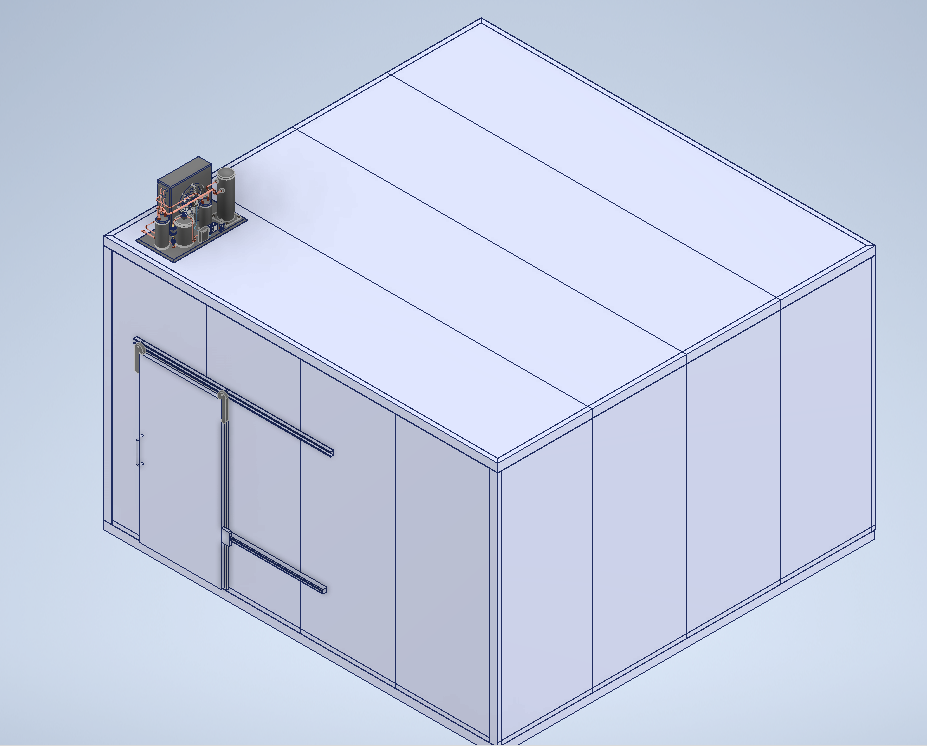
\includegraphics[width=0.6\linewidth]{figures/final1}
	\caption{Diseño preliminar final, vista frontal}
	\label{fig:final1}
\end{figure}



\begin{figure}[H]
	\centering
	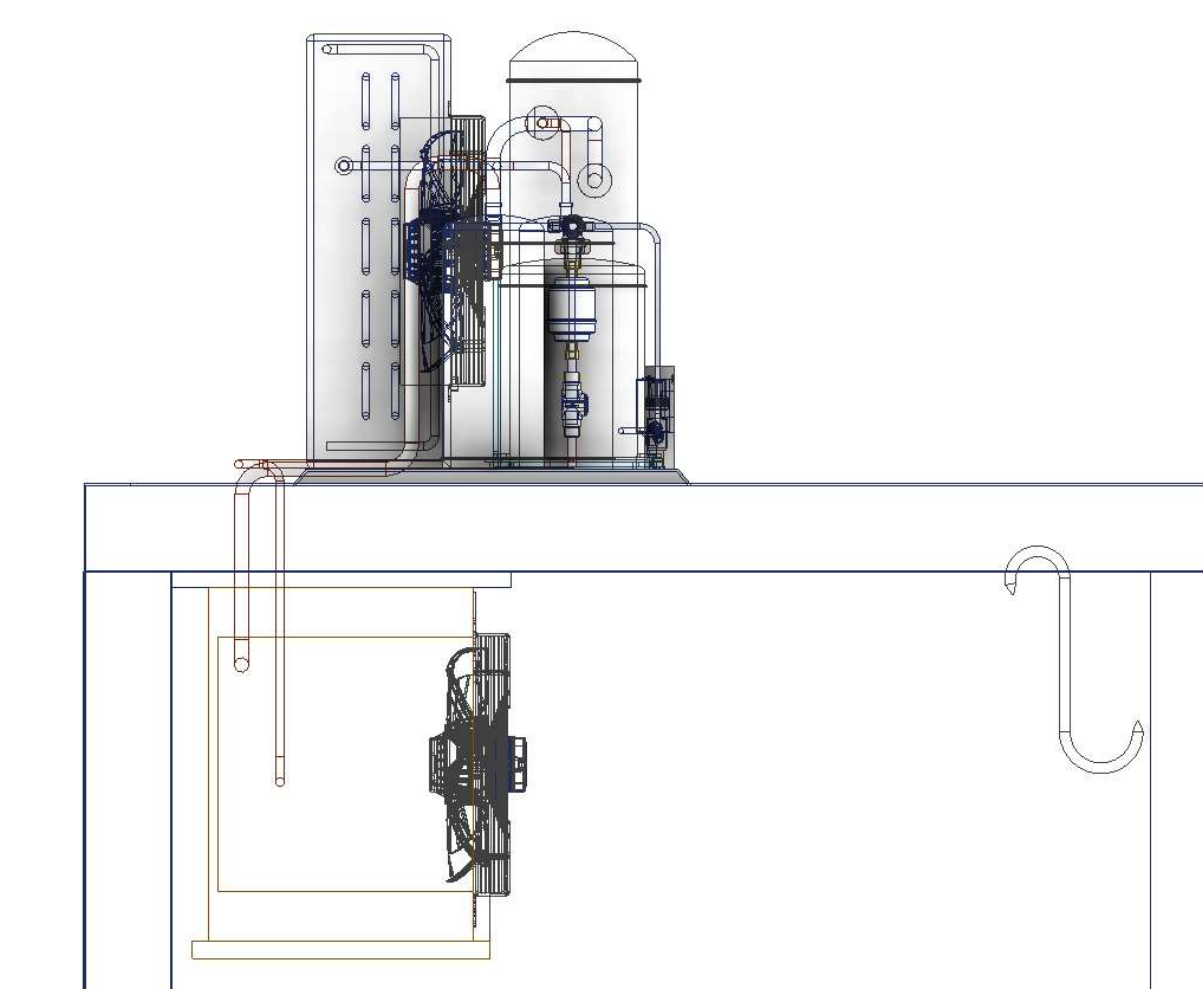
\includegraphics[width=0.6\linewidth]{figures/axo-design-cableado}
	\caption{Vista de la cámara con el diseño final nivel de cableado}
	\label{fig:plano-fin}
\end{figure}


\begin{figure}[H]
	\centering
	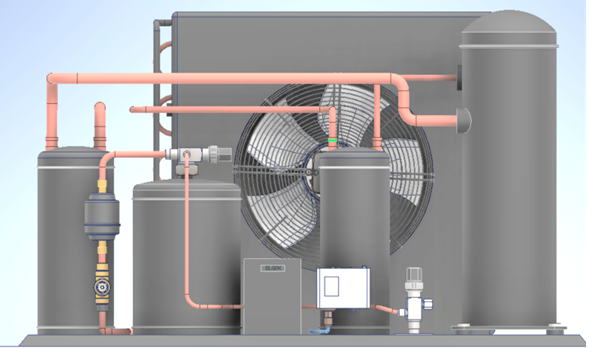
\includegraphics[width=0.46\linewidth]{figures/design-enfria}
	\caption{Sistema de ventilación}
	\label{fig:design-enfria-fin}  Fuente: Elaboración propia basado de \citeNP{bibliocad}
\end{figure}

\begin{figure}[H]
	\centering
	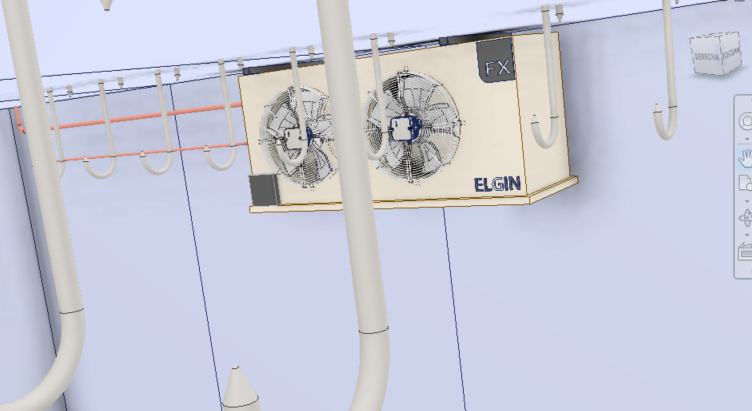
\includegraphics[width=0.46\linewidth]{figures/design-ventils}
	\caption{Vista interior de la cámara de refrigeración (Sistema de ventilación )}
	\label{fig:design-ventils}  Fuente: Elaboración propia basado de \citeNP{bibliocad}
\end{figure} 
Consulte los anexos gráficos  para ver más detalles de los planos y del diseño.



\begin{table}[H]
	\centering
	\caption{Elementos principales seleccionados de forma general del sistema.}
	Fuente: Elaboración propia basada en \cite{caterpillar-2008}
	\begin{tabular}{cccc}
		\hline
		\textbf{Num} & \textbf{Nombre del componente} & \textbf{Material}                                                         & \textbf{Marca} \\ \hline
		1               & Paneles superiores (techo)                & \begin{tabular}[c]{@{}c@{}}Acero inoxidable con \\ aislamiento de poliuretano\end{tabular}  & Kingspan                 \\
		2               & Paneles laterales (paredes)               & \begin{tabular}[c]{@{}c@{}}Acero galvanizado con\\  aislamiento de poliuretano\end{tabular} & Metecno                  \\
		3               & Puertas/ventanas                          & \begin{tabular}[c]{@{}c@{}}Acero inoxidable con \\ aislamiento térmico\end{tabular}         & True                     \\
		4               & Evaporador                                & Aluminio                                                                                    & Alfa Laval               \\
		5               & Condensador                               & Cobre y aluminio                                                                            & Emerson                  \\
		6               & Compresor                                 & Acero                                                                                       & Copeland                 \\
		7               & Válvula de expansión                      & Latón                                                                                       & Danfoss                  \\
		8               & Recubrimiento lateral                     & Acero inoxidable                                                                            & Kingspan                 \\
		9               & Recubrimiento superior                    & Acero inoxidable                                                                            & Metecno                  \\ \hline
	\end{tabular}
	\label{tabla:lista-componentes-fin}
\end{table}


\newpage
\section{Conclusión}

En este capítulo se han atacado los planteamientos básicos del diseño y la implementación de una cámara de refrigeración para conservar insulina en la Ciudad de México, los cuales sin duda, son procesos complejos que demandan una atención meticulosa a diversos aspectos. Además de los aspectos técnicos y logísticos, es fundamental adoptar un enfoque integral que considere las necesidades y preocupaciones de los pacientes diabéticos, así como el impacto potencial en la salud pública.\\ 
Además de garantizar la calidad y la eficacia de la insulina almacenada, es importante prestar atención a la disponibilidad y accesibilidad de la insulina para los pacientes diabéticos. Esto incluye aspectos como la distribución eficiente de los medicamentos, la gestión de inventarios y la coordinación con las unidades de atención médica para garantizar un suministro continuo y adecuado. \\
Por otro lado, conocer los planos y bosquejos preliminares es crucial para garantizar el almacenamiento seguro y eficiente de medicamentos sensibles, como la insulina. Permiten la identificación de áreas críticas, como la distribución de unidades de refrigeración, el aislamiento térmico adecuado y los sistemas de monitoreo y control de temperatura.\\ 
Adicionalmente, la selección adecuada de los materiales es esencial para asegurar la durabilidad, eficiencia y seguridad de la cámara de refrigeración. Materiales como el acero inoxidable y el aluminio no solo ofrecen resistencia a la corrosión y excelentes propiedades térmicas, sino que también contribuyen a la sostenibilidad del sistema al ser reciclables.\\ 
Finalmente, la etapa de ecodiseño es crucial para minimizar el impacto ambiental a lo largo del ciclo de vida de la cámara de refrigeración. Esto implica la consideración de factores como el consumo energético, la selección de materiales sostenibles y la eficiencia de los procesos de fabricación y reciclaje.\\
Un enfoque de ecodiseño no solo contribuye a la conservación del medio ambiente, sino que también puede generar beneficios económicos a largo plazo al optimizar recursos y reducir costos operativos.





